\documentclass[a4paper]{report}
\usepackage[latin1]{inputenc}
\usepackage[english]{babel}
\usepackage[T1]{fontenc}
\usepackage[bottom]{footmisc}
\usepackage{graphicx}
\usepackage{newlfont}
\usepackage{xcolor}
\usepackage{colortbl}
\usepackage{booktabs}
\usepackage{mathdots}
\usepackage{amssymb}
\usepackage{amsmath,amssymb}
\usepackage{amsmath}
\usepackage{enumerate}
\usepackage{amsmath,accents}


\textwidth=450pt\oddsidemargin=0pt
\pagestyle{plain}

\newcommand\tab[1][1cm]{\hspace*{#1}}

\begin{document}
     \begin{titlepage}
		\begin{center}
			{{\Large{\textsc{Politecnico di Milano}}}} \rule[0.1cm]{15.8cm}{0.1mm}
			\rule[0.5cm]{15.8cm}{0.6mm}
			{\small{\bf School of Industrial and Information Engineering\\
					M.Sc. of Mathematical Engineering\\
					Computational Science and Engineering}}
		\end{center}
		\begin{center}
			
\includegraphics[scale=0.2]{poli}
		\end{center}
		\vspace{25mm}
		\begin{center}
			{\LARGE{\bf Mixed Finite Element Methods for }}\\
			\vspace{3mm}
			{\LARGE{\bf Coupled 3D/1D Fluid Curved Problem}}\\
			\vspace{25mm} {\large{\bf {Project of Advance Programming for Scientific Computing}}}\\
			\vspace{25mm} {\large{\bf {Giorgio Raimondi}}}\\
			\large{\bf Matr. 853037}\\
		\end{center}
		\vspace{30mm}
		\begin{center}
			{\large{\bf $\bullet$ May 2017 $\bullet$ \\
					Accademic Year 2016/2017 }}
		\end{center}
	\end{titlepage}



\tableofcontents
 
 
\addcontentsline{toc}{chapter}{Introduction}
\chapter*{Introduction}
\setcounter{page}{1} 
The main goal of this project is to develop a general-purpose finite element solver for large scale simulation of microcirculation for a generic network geometry.In particular we want to extend the previous models, which are able to solve the problem only for rectilinear networks, to one able to take in account the presence of curved branches.\\
Thanks to dimensional model reduction techniques, the vessel tree is described as a one-dimensional (1D) manifold immersed in a three-dimesional (3D) interstitial volume. Vessels can be seen as concentrated sources lead to reduce the computational cost of simulations. However, concentrated sources lead to singular solutions that still require computationally expensive meshes to guarantee accurate approximation. The main computational barrier consists in the ill-posedness of restriction operators applied on manifolds with co-dimension larger than one. We overcome the computational challenges of approximating PDEs on manifolds with high dimensionality gap by means of nonlocal restriction operators that combine standard trace with mean values of the solution on low dimensional manifolds.\\



\newpage
\chapter{Coupled 3D/1D Problem}
	\section{Model set up}
	The domain in $\mathbb{R}^{3} $ where the model is defined is composed by two parts, $\Omega_{t}$ and $\Omega_{v}$, denoting the interstitial volume and the vessel bed respectively. Assuming thet the vessels can be described as cylindrical tubes, we denote with $    	\Gamma$ the outer surface of $\Omega_{v}$ while $\Lambda$ indicates the 1D manifold representing the vessel centerline. The vessel radius R is generally subject to change in the network.\newline
	We consider the interstitial volume $\Omega_{t}$ as an isotropic porous medium, descibed by the Darcy's law. Ignoring inertial and body forces, it reads:
\begin{equation}
\mathbf{u}_{t} =  -\frac{1}{\mu}\boldsymbol{\mathbb{K}}\nabla p_{t} 
\end{equation}

where $\mathbf{u}_{t}$ is average filtration velocity vector in the tissue, $\boldsymbol{\mathbb{K}}$ is the permeability tensor, $\mu$ is the viscosity of the fluid and $p_{t}$ is the fluid pressure. Recall that in the simple isotropic case the permeability tensor is given by $\boldsymbol{\mathbb{K}}=k\boldsymbol{\mathbb{I}}$, being $ k$ the scalar permeability and $\boldsymbol{\mathbb{I}}$ the identity tensor. \\

\indent Concerning  the vessels, we start assuming a steady incompressible Navier-Stokes model for blood flow, namely:
\begin{equation}
\rho (\mathbf{u}_{v}\cdot \bigtriangledown)\mathbf{u}_{v} - \mu \bigtriangleup\mathbf{u}_{v} +\bigtriangledown p_{v} =0
\end{equation}
where $\mathbf{u}_{v}$ is the flow velocity, $p_{v}$ is the pressure and $\rho$ the density of the fluid.
		\begin{center}
			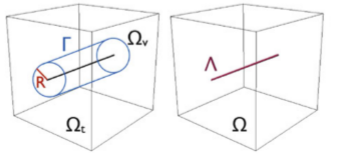
\includegraphics[scale=1]{domain}
		\end{center}




\section{Coupling microcirculation with interstitial flow}
	At this stage the two problems are completely uncorrelated. Indeed to close the problem we need to impose the continuity of the flow at interface $\Gamma=\partial \Omega_v \cap \partial \Omega_t$, namely:
\begin{equation}
\mathbf{u}_{v} \cdot \mathbf{n} = \mathbf{u}_{t} \cdot \mathbf{n} = L_{p} ( p_{v} - p_{t} ) ,   \mathbf{u}_{v} \cdot \boldsymbol{\tau} = 0 ,
\end{equation}
where $\mathbf{n}$ and $\boldsymbol{\tau}$ are the outward unit normal vector and the unit tangent vector on surface $\Gamma$, respectively, while $L_{p}$ is the hydraulic conductivity of the vessel wall.
This equation together to the previous ones identify a fully three-dimensional model able to capture approximation of the phenomena we are interested in. However, many technical difficulties arise in the numerical approximation of the coupling between a complex network with surrounding volume. To this purpose, we adopt the multiscale approach to avoid the complex 3D geometry of the network. We exploit the {\it Immersed Boundary Method (IBM)} combined with the assumption of large aspect ratio between vessel radius and capillary axial length. More precisely, we apply a suitable rescaling of the equation and let the capillary radius go to zero ($ R \rightarrow 0$).\newline
As a consequence, the three-dimensional description of the vessels is reduced to a simplified one-dimensional representation by replacing the immersed interface and the related interface conditions with an equivalent mass source, namely:
\begin{equation}
 \mathbf{u}_{t} \cdot \mathbf{n} =f ( p_{v} , p_{t} )\quad on \quad \Gamma ,
\end{equation}
being $f$ the flux per unit area released through surface $\Gamma$: it is a point-wise constitutive law for the capillary leakage in term of the fluid pressure.



	\section{Derivation of the 1D approximation in case of rectilinear axis}
Here we introduce the simplest non-linear 1D flow in compliant vessels.\newline
The basic equations are derived for a track of vessel free of bifurcations, which is idealised as a cylindrical compliant tube.\newline
We will mainly use the Cartesian coordinates, but when dealing with cylindrical geometries it is handy to introduce a cylindrical coordinate system. Therefore, in the following we indicate with $\boldsymbol{\epsilon}_{r}$, $\boldsymbol{\epsilon}_{\theta}$ and $\boldsymbol{\epsilon}_{z}$ the radial circumferential and axial unit vectors, respectively, $(r,\theta,z)$ being the corresponding coordinate.


\subsection{Model Assumptions}
The basic model is deduced by making the following assumptions:
\begin{enumerate}
	\item \textbf{Axial symmetry.} All quantities are independent from the angular coordinate $\theta$. As a consequence, every axial 	section $z=const$ is assumed circular on all the vessel. The tube radius $R$ is a function of $z$.
	\item \textbf{Fixed cylinder axis.} This simply means that the axis is assumed as rectilinear for the whole vessel. This hypothesis is indeed consistent with that of axial symmetry.
	\item \textbf{Constant pressure on each section.} We assume that the pressure $P$ is constant on each section. This comes as result of the following count:\\
using the axial symmetry we have $\mathbf{u}_{v}(r,\theta,z)=u_{z}(r,\theta,z) \boldsymbol{\epsilon}_{z}$ and splitting the equation $[1.2]$ by components we obtain
		\begin{equation}
			\begin{cases}
				(\mathbf{u} \cdot \nabla) u_{r} - \nu \triangle u_{r}+\partial_{r} p / \rho = 0\\
				(\mathbf{u} \cdot \nabla) u_{\theta} - \nu \triangle u_{\theta}+\partial_{\theta} p / \rho = 0\\
				(\mathbf{u} \cdot \nabla) u_{z} - \nu \triangle u_{z}+\partial_{z} p / \rho = 0\\
			\end{cases} \quad
		\Rightarrow \quad
			\begin{cases}
				\partial_{r} p = 0\\
				\partial_{\theta} p = 0\\
				\rho (\mathbf{u} \cdot \nabla) u_{z} -\mu \triangle u_{z} + \partial_{z} p = 0
			\end{cases}
		\end{equation}
		So we see that $p$ depends only on $z$.
	\item \textbf{No body forces.} We neglect body forces.
	\item \textbf{Dominance of axial velocity.} The velocity components orthogonal to the $z$ axis are negligible compared to the component along $z$. The latter is indicate by $u_{z}$ and its expression in cylindrical coordinates is supposed to be of the form
		\begin{equation}
			u_{z}(r,z) = \overline{u} (z)  s(r R^{-1}(z))
		\end{equation}
	where $\overline{u}$ is the mean velocity on each section, $s: \mathbb{R}\rightarrow \mathbb{R}$ is the velocity profile and reads as
		\begin{equation}
			s(y)= \gamma^{-1} (\gamma + 2) (1+y^{\gamma}).
		\end{equation}
\end{enumerate}
The fact that the velocity profile does not vary in space is in contrast with experimental observations and numerical results carried out with full-scale models. However, it is a necessary condition for the derivation of the reduced model. One may think to $s$ as being a profile representative of an average flow configuration.\\
		\begin{center}
			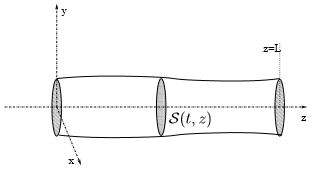
\includegraphics[scale=1]{tubo_dritto}
		\end{center}
A generic axial section will be indicated by $S=S(z)$. Its measure $A$ is given by
	\begin{equation}
		A(z) =\int_{S(z)} d\sigma = \pi R^{2}(z).
	\end{equation}
The mean velocity $ \overline{u}$ is given by
	\begin{equation}
		\overline{u}=A^{-1} \int_{S} u_{z} d\sigma.
	\end{equation}
We will indicate with $\alpha$ the momentum-flux correction coefficient, (sometimes also called Coriolis coefficent) defined as
	\begin{equation}
		\alpha = \frac{\int_{S} u_{z}^{2} d\sigma}{A \overline{u}^{2}}= \frac{\int_{S} s^{2} d\sigma}{A}
	\end{equation}
where the dependence of various quantities on the spatial coordinates is easy to understand. In general this coefficient will vary in time and space, yet in our model it is taken constant as a consequence of [1.6].




\subsection{Model Derivation }
To derive our model, we use an approach consisting of integrating the Navier-Stokes equations on a generic portion P of the vessel. Moreover we can provide the vessel wall in parametric form:
	\begin{equation}
		\Gamma=\{ (r,\theta,z): r=R(z), \theta \in [0,2\pi), z \in (0,L) \}
	\end{equation}
where L is the length of the vessel in the axial direction and \textbf{n} is the out oriented normal to $\partial \Omega_v$.\\
Under the previous assumption, the momentum along z and continuity equations, in the hypothesis of constant viscosity, are
	\begin{equation}
		\begin{cases}
			\rho (\mathbf{u} \cdot \nabla) u_{z} - \mu \triangle u_{z} + \partial_{z} p =0 \\
			div \mathbf{u} = 0
		\end{cases}
	\end{equation}
The convective term in the momentum equation has been taken in divergence form because it simplifies the further derivation.
Now we are ready to derive our reduced model and we start first from the continuity equation
	\begin{equation}
		\begin{split}
		0=\int_P[ div \mathbf{u}] d\Omega \quad= \int_{\partial P}[\mathbf{u} \cdot \mathbf{n} ]d\sigma \quad =\int_{S(z_1)} [\mathbf{u} \cdot \mathbf{n} ]d\sigma \quad + \int_{S(z_2)}[ \mathbf{u} \cdot \mathbf{n}] d\sigma \quad + \int_{\Gamma}[ \mathbf{u} \cdot \mathbf{n}] d\sigma \quad =\\
= -\int_{S(z_1)} [u_z] d\sigma \quad+\int_{S(z_2)}[ u_z] d\sigma \quad+ \int_{\Gamma}[ f(\overline{p}_{t},p_{v})]  d\sigma
		\end{split}
	\end{equation}
using the fact that $\mathbf{n}=\boldsymbol{\epsilon_{z}}$ on $S(z_1)$ and $S(z_2)$ and the equation [1.4]. Now using equation [1.9]  for the first two integrals and a change of variable on the third one we obtain:
	\begin{equation}
		\begin{split}
	[1.13]= -\overline{u}(z_1) A(z_1) + \overline{u}(z_2) A(z_2) + \int^{z_2}_{z_1}[ f(\overline{p_t},p_v)] dz = \\
		=  \int^{z_2}_{z_1}[ f(\overline{p_t},p_v) + \partial_z (A \overline{u})] dz
		\end{split}
	\end{equation}
since $\overline{p_t} = \frac{1}{2 \pi R}\int_{\partial S} p_t ds$ is the mean interstitial pressure on the boundary of a section $S$ and the fundamental theorem of calculus hold. At the end we use the arbitrary of  $z_1$ and $z_2$ to obtain
	\begin{equation}
	\partial_{z}(A \overline{u})+f(\overline{p_t},p_v)=0
	\end{equation}

Now it's the turn of the momentum equation. Lets start with the Stokes term:
	\begin{equation}
	\int_{P}[\partial_{z}p]d\Omega=\int_{z_1}^{z_2}dz\int_{S(z)}	[\partial_z p] d\sigma=\int_{z_1}^{z_2} [A(z) \partial_z p]dz
	\end{equation}
Now we manipulate the advective term in divergence form:
	\begin{equation}
	\int_P [div(u_z \mathbf{u})]d\Omega =	\int_{\partial P} [u_z \mathbf{u} \cdot \mathbf{n}]d\sigma = -\int_{S(z_1)} [u_z^2]d\sigma + \int_{S(z_2)}[u_z^2]d\sigma + \int_{\Gamma} [u_z \mathbf{u} \cdot \mathbf{n}]d\sigma
	\end{equation}
In order to eliminate the boundary integral we exploit the fact that $u_z=0 $ on $\Gamma$. Subsequently using equation [1.10] and the fundamental theorem of calculus we obtain:
	\begin{equation}
	-\int_{S(z_1)}[u_z^2]d\sigma+\int_{S(z_2)}[u_z^2]d\sigma = \alpha[-\overline{u}(z_1)^2 A(z_1)+\overline{u}(z_1)^2 A(z_1)]=\int_{z_1}^{z_2}\alpha \partial_z[A(z)\overline{u}(z)^2]dz
	\end{equation}
We finally consider the viscous term:
	\begin{equation}
		\int_P [\triangle u_z]d\Omega = \int_{\partial P}[\nabla u_z \cdot \mathbf{n}]d\sigma =-\int_{S(z_1)}[\partial_z u_z]d\sigma+\int_{S(z_2)}[\partial_z u_z]d\sigma+\int_{\Gamma}[\nabla u_z \cdot \mathbf{n}]d\sigma.
	\end{equation}
Here, we neglect the $ \partial_z u_z $ term by the fact that $ 0=div(\mathbf{u})=\partial_z u_z$ almost everywhere in $\Omega_v$. Moreover we split the $\mathbf{n}$ vector into two components, the radial component $\mathbf{n}_r=(\mathbf{n} \cdot \boldsymbol{\epsilon}_r)\boldsymbol{\epsilon}_r =n_r \boldsymbol{\epsilon}_r$ and axial component $\mathbf{n}_z= \mathbf{n}-\mathbf{n}_r$. Remember that owing to the cylindrical geometry, $\mathbf{n}$ has no component along the circumferential coordinate and, consequently, $\mathbf{n}_z$ is indeed oriented along z. Thus, we can write:
\begin{equation}
\int_P [\triangle u_z] d\Omega= \int_{\Gamma}[\nabla u_z \cdot \mathbf{n}_r+\nabla u_z \cdot \mathbf{n}_z]d\sigma.
\end{equation}
Again, we neglect the $\nabla u_z \cdot \mathbf{n}_z$, which is proportional to $\partial_{z} u_z $. We recall now the relation [1.6] to write:
\begin{equation}
\int_{\Gamma} [\nabla u_z \cdot \mathbf{n}_r]d\sigma = \int_{\Gamma}[n_r \nabla u_z \cdot \boldsymbol{\epsilon}_r]d\sigma=\int_{\Gamma}[\overline{u} R^{-1}s'(1) n_r]d\sigma = \int_{z_1}^{z_2}[2\pi s'(1)  \overline{u}]dz
\end{equation}
where we used $n_r d\sigma= 2\pi R dz$ and indicating $s'$ as the first derivative of s.
Then using the arbitrary of the extreme on [1.16], [1.18], [1.21] and calling $K_r= 2\pi \nu s'(1)$ we obtain
\begin{equation}
K_r \overline{u}+ \frac{A}{\rho} \partial_{z} p + \alpha \partial_z (A \overline{u}^2)=0
\end{equation}



\subsection{Full linear coupled equations}
Now that we have derived the 1D model equatiosn we need to generalize them to a more complex topology.
To this purpose, we decompose the network in $\Lambda_i$ branches, $i=1,...,N$. The branches are parametrized by the arc length $s_i$; a tangent unit vector $\boldsymbol{\lambda}_i$ is also defined over each branch, accounting for an arbitrary branch orientation. Differentiation over the branches is defined using the tangent unit vector, namely $\boldsymbol{\partial}_{s_i}:=\nabla \cdot \boldsymbol{\lambda}_i$ on $\Lambda_i$, i.e. $\boldsymbol{\partial}_{s_i}$ represents the projection of $\nabla$ along $\boldsymbol{\lambda}_i$.\\
So the coupled 3D-1D problem we have to solve, in case of vessel with rectilinear axis, is:
\begin{equation}
\begin{cases}
\quad \mathbf{u}_t + \frac{1}{\mu} \boldsymbol{\mathbb{K}} \nabla p_t =0 &  on \quad \Omega_t\\
\quad  div(\mathbf{u}_t)- 2 \pi R L_p (p_v -\overline{p_t}) \delta_{\Lambda}=0& on \quad \Omega_t\\
\quad  K_r \overline{u}+ \frac{A}{\rho} \partial_{z} p + \alpha \partial_z (A \overline{u}^2)=0& on \quad \Omega_v \\
\quad 	\partial_{z}(A \overline{u})+2 \pi R L_p (p_v -\overline{p_t})=0 & on \quad \Omega_v
\end{cases}
\end{equation}

\subsection{Boundary conditions}
For the well-poseness of problem [1.23], we have to specify suitable boundary conditions ($\mathbf{BC}_s$) on both the tissue and vessel boundary, i.e. $\partial \Omega$ and $\partial \Lambda$ respectively.\\
Since we aim to present the most generic setting, we assume the tissue interstitium boundary to be partitioned as follows:
\begin{equation}
\partial \Omega= \Gamma_p \cup \Gamma_u, \quad \mathring{\Gamma}_p \cap \mathring{\Gamma}_u=\emptyset.
\end{equation}
As suggested by the apices $p$ and $u$, we enforce a given pressure distribution on $\Gamma_p$ and/or a fixed value for the normal flux over $\Gamma_u$, namely:
\begin{align}
p_t=g_t \quad & \quad on \quad \Gamma_p,\\
\mathbf{u}_t \cdot \mathbf{n}=\beta (p_t - p_0 ) \quad & \quad on\quad \Gamma_u,
\end{align}
Here $p_0$ represent far field pressure value, while $\beta$ can be interpreted as an effective conductivity accounting for layers of tissue surrounding the considered sample. Assuming that the interstitial pressure decay from $p_t$ to $p_0$ over a distance comparable to the sample characteristic size, $D$, dimensional analysis shows that a rough estimate of conductivity is $\beta= k_t/D$. For the pressure datum we require $g_t \in L^2(\Gamma_p)$.\\
Concerning the network, we split the collection of extrema into two subset: on the \textit{boundary extrema}, $\boldsymbol{\varepsilon}_p$, we enforce a pressure distribution, on \textit{immersed extrema} ,  $\boldsymbol{\varepsilon}_u$, we enforce the flux (hence the vessels velocity); namely:
\begin{align}
 p_v=g_v \quad \quad & \quad \quad on \quad \boldsymbol{\varepsilon}_p\\
\pi R'^2 u_v =\beta (p_v-p_0)&\quad \quad on \quad \boldsymbol{\varepsilon}_u
\end{align}
where $g_v$ is a boundary datum for which is required measurability and square-summability, namely $g_v \in L^2(\boldsymbol{\varepsilon}_p)$, while $p_0$ and $\beta$ are as above. In particular, in future applications we will always enforce constant pressure drop $P^{out}_v-P^{in}_v$, that means we will adopt piecewise-constant boundary data.




\section{Derivation of the 1D approximation for curved segments}
\subsection{Preliminary Model  Assumptions}
Now we want to derive similar results in the case of curvilinear axis.\\
To do this we define the parametric arc length $\boldsymbol{\Psi}: \mathbb{R} \rightarrow \mathbb{R}^3$ as the axis trajectory, taken such that
\begin{equation}
\begin{split}
\boldsymbol{\Psi} \in C^3(\mathbb{R}) \\
| \boldsymbol{\Psi} ' (z) | = 1 \quad \forall z \in [0,L],
\end{split}
\end{equation}
where $L$ is the length of the arc  and the norm is compute as the Euclidean norm.
In the following we will use parametric cylindrical coordinate, and we indicate $\boldsymbol{\epsilon}_{r(z)}$, $\boldsymbol{\epsilon}_{\theta(z)}$ and $\boldsymbol{\epsilon}_{\psi(z)}$ respectively, the radial, circumferential and axial unit vectors, $(r,\theta,\psi)(z)$ being the corresponding coordinates at each position $z$ and, due to the choose of $\boldsymbol{\Psi}$, we obtain that $\boldsymbol{\psi (z)}=\boldsymbol{\Psi}'(z)$.
From now on we will omit the parametric dependence.
To derive the model we need these preliminary assumptions:
	

	\begin{enumerate}
	\item\textbf{Circular Section.} For each value of the parameter $z$ the intersection between the orthogonal plane to $\boldsymbol{\psi }$ and the vessel wall is assumed as circular.
	\item \textbf{Constant pressure on each section.} The pressure is assumed constant on each section due to the same reason of the rectilinear case.
	\item \textbf{No body forces.} We neglect all forces effect.
	\item \textbf{Dominance of axial velocity.} The velocity components orthogonal to the $\psi$  axis are negligible compared to the component along $\psi$. The latter is indicate by $u_{\psi}$ and its expression is supposed to be of the form:
	\begin{equation}
 	u_{\psi}(r,\theta,\psi)= \overline{u}(\psi) \Phi (r,\theta,\psi),
	\end{equation}
where $\overline{u}$ is the mean velocity on each axial section and $\Phi :\mathbb{R}^3 \rightarrow \mathbb{R}$ is the velocity profile on the curvilinear vessel. As for the linear case, this profile can also be seen as the average flow configuration.
	\end{enumerate}




\subsection{Derivation of the average velocity profile}
To derive the velocity profile we are going to study it in the simpler case of a curve vessel with fixed curvature and we will generalize it in a more complete problem adding more hypothesis.
		\begin{center}
			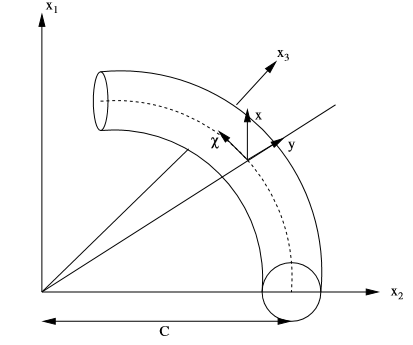
\includegraphics[scale=0.7]{tubo_curvo}
		\end{center}
Surely there are many possible ways to choose the configuration of $\Phi$, but we are going to use the following second order approximation:
\begin{equation}
\Phi (r,\theta, \psi) = s(r R^{-1}) (1+ a r \cos \theta+ b r \sin \theta + c r^2 \cos \theta \sin \theta + d r^2 \cos^2 \theta + e r^2 \sin^2 \theta),
\end{equation}
where $a$,$b$,$c$,$d$ and $e$ are constants depending on the curvature and $s$ is the velocity profile of the linear case. To improve the significance of this configuration is possible to add higher order term and compute the respectively coefficients.\\
Now to better understand the procedure, let's take for example a uniform curvilinear motion. On it we have that the tangential velocity is proportional to the distance from the center, so in out problem we are going to expect similar result.\\
Given $\kappa$, the curvature of the arc, defined as $\kappa = |\boldsymbol{\Psi}''|$, and the centripetal unitary direction $\mathbf{N}=\boldsymbol{\Psi}''/\kappa$, we have that the center $C_0$ of the {\it osculating circle} is the point in direction $\mathbf{N}(z)$ whose distance from $\boldsymbol{\Psi} (z)$ is $R_0$, where $R_0$ is the curvature radius and it's equal to $1/\kappa$.
		\begin{center}
			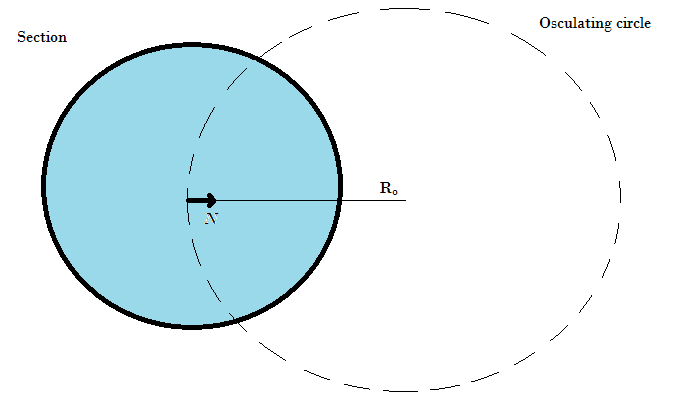
\includegraphics[scale=0.4]{Osculator_circle}
		\end{center}
Now we have to impose suitable condition to our velocity profile in order to compute the value of all the constants:
	\begin{enumerate}	
	\item \textbf{Choice of $\theta$.} To simplify our calculation we assume that on each section all the vectors with $\theta=0$ are in $\mathbf{N}$ direction.
	\item \textbf{Symmetry of the profile.} In each section the profile must be symmetric with respect to the axes connecting $C_0 $ and $\boldsymbol{\Psi}(z)$. So:
	\begin{equation*}
		\Phi (r,\theta, \psi)= \Phi(r, -\theta, \psi) \quad \forall r,\theta,\psi
	\end{equation*}
and we obtain that $b=c=0$.
	\item\textbf{Zero velocity in the Center.} For the linear dependence of the velocity with the distance from the center of the osculating circle, our profile must be zero in $C_0 = (r=1/\kappa, \theta=0, \psi).$
	\begin{equation*}
	\Phi (C_0)= 0 \rightarrow (1+a/\kappa+d/\kappa^2)=0 	\rightarrow d=-a\kappa - \kappa^2
	\end{equation*}
	\item \textbf{Linear dependence.} Due to the assumptions that the velocity profile is linear dependent to the distance from the center of the osculating circle we have that all the points with distance $1/\kappa$ from it must have the same dependence.\\
All these are the points having the following property:
\begin{equation*}
\phi=\{(r,\theta): \quad r= \frac{2 \cos \theta}{\kappa}, \quad \theta \in [-\frac{\pi}{2}; +\frac{\pi}{2}] \}.
\end{equation*}
Moreover we have that
\begin{equation*}
\Phi(r=0,\theta,\psi)= s(0)
\end{equation*}
so $\forall (r,\theta) \in \phi$ then $\Phi(r,\theta, \psi)= s(r/R)$. It follows that $\forall (r,\theta) \in \phi$:
\begin{equation*}
0 = a r \cos \theta + d r^2 \cos^2 \theta + e r^2  \sin^2 \theta = 2 \frac{a}{\kappa} \cos^2 \theta + 4 \frac{d}{\kappa^2} \cos^4 \theta + 4 \frac{e}{\kappa^2} \cos^2 \theta \sin^2 \theta .
\end{equation*}
Now for $\theta=\pm \frac{\pi}{2}$ the equation is verified. In the other cases we can divide all by $2 \cos^2 \theta / \kappa^2$, to obtain:
\begin{equation*}
0= a \kappa + 2 d \cos^2 \theta + 2 e \sin^2 \theta \quad \quad \forall 	\theta  \in (-\frac{\pi}{2};+\frac{\pi}{2}).
\end{equation*}
To find the value of the constant, we test it on two particular cases: $\theta= \pi/4, \theta= \pi/3$.\\
For $\theta=\pi/4$, using assumption 3:
\begin{equation*}
0=a \kappa + 2d (\frac{1}{2})+ 2 e(\frac{1}{2})= a\kappa + d+ e = a\kappa -\kappa^2 -a\kappa + e=e-\kappa^2 .
\end{equation*}
For that $e=\kappa^2$.
Instead for $	\theta= \pi/3$, using assumption 3 and the previous result:
\begin{equation*}
0= a \kappa + 2 d(\frac{1}{4})+ 2 e(\frac{3}{4})= a\kappa + \frac{d}{2}+ \frac{3e}{2}= a\kappa-\frac{ \kappa^2}{2}-\frac{a\kappa}{2}+\frac{3 \kappa^2}{2}= \frac{a\kappa}{2}+\kappa^2
\end{equation*}
So $a= -2\kappa$ and $d=\kappa^2$.
	\end{enumerate}

Due to this assumptions, our velocity profile is of the form:
\begin{equation}
\Phi(r,\theta,\psi) = s(r R^{-1})(1+r^2 \kappa^2- 2\kappa r \cos \theta).
\end{equation}
In a general geometry we have that the curvature is dependent on the trajectory position: $\kappa= \kappa (\psi)$.
But thanks to the assumption of regularity on the trajectory, $\boldsymbol{\Psi} \in C^3(\mathbb{R})$, then $\kappa(\psi) \in C^1(\mathbb{R})$ and our velocity profile still holds, by continuity of $\kappa$:
\begin{equation}
\Phi(r,\theta,\psi) = s(r R^{-1})(1+r^2 \kappa^2(\psi)- 2\kappa(\psi) r \cos \theta).
\end{equation}

\newpage
\begin{figure}[htbp]
\centering
\begin{minipage}[c]{.30\textwidth}
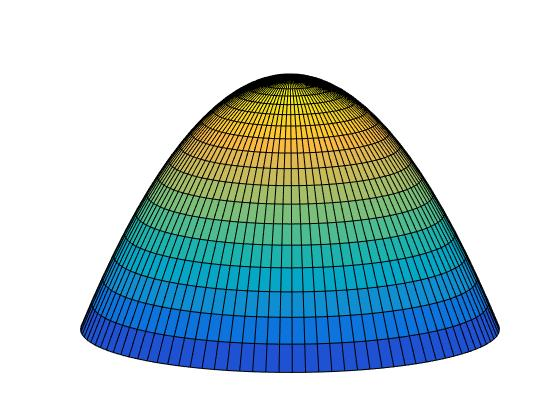
\includegraphics[width=.70\textwidth]{k0}
\caption{$\kappa R=0$}
\end{minipage}%
\hspace{10mm}%
\begin{minipage}[c]{.30\textwidth}
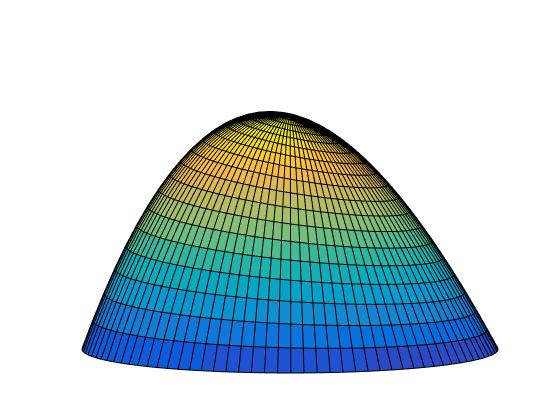
\includegraphics[width=.70\textwidth]{k01}
\caption{$\kappa R=0.1$}
\end{minipage}% 
\\
\begin{minipage}[c]{.30\textwidth}
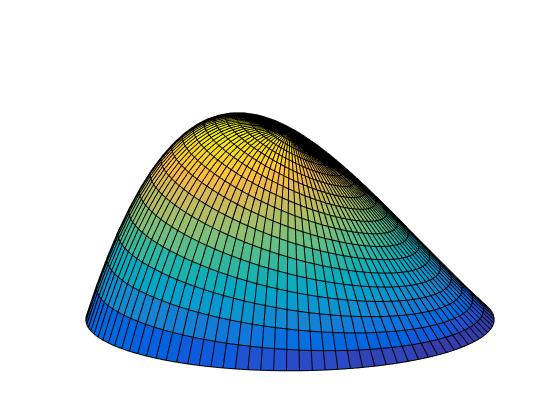
\includegraphics[width=.70\textwidth]{k03}
\caption{$\kappa R=0.3$}
\end{minipage}%
\hspace{10mm}%
\begin{minipage}[c]{.30\textwidth}
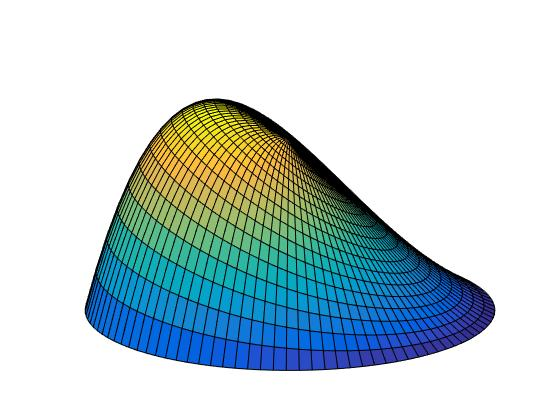
\includegraphics[width=.70\textwidth]{k05}
\caption{$\kappa R=0.5$}
\end{minipage}%
\\
\begin{minipage}[c]{.30\textwidth}
\includegraphics[width=.70\textwidth]{k1}
\caption{$\kappa R=1.0$}
\end{minipage}
\caption{Velocity profile with imposition of Poiseuille flow ($\gamma =2$) for different curvature value. As we can see from these plots, we have that for increasing curvature value, the velocity profile on the section starts to concentrate farther from the center of the osculating circle.}
\end{figure}



\subsection{Model derivation for curved segments}
Now that we have the velocity profile, the derivation of the equation is the same of the rectilinear case, the only difference is for the coefficients which depend on the profile.\\
In fact the integral of an integrable  function $f: \mathbb{R}^3 \rightarrow \mathbb{R}$ on trajectory $\boldsymbol{\Psi}$ is
\begin{equation}
\int_{\boldsymbol{\Psi}} [f(\psi) ] d\psi =\int_0^L [f(\boldsymbol{\Psi}(z)) |\boldsymbol{\Psi}'|]dz=\int_0^L [f(\boldsymbol{\Psi}(z))] dz.
\end{equation}
To denote our portion P we can use two arbitrary position $z_1$ and $z_2$ $\in$ $[0,L]$, $z_1<z_2$ and we obtain the same results.\\
The first difference is on equation [1.10]:
\begin{equation*}
\alpha^{**}= \frac{\int_S [u_{\psi}^2] d\sigma}{A \overline{u}^2}=\frac{\int_S [\Phi^2]d\sigma}{A}= \frac{\int_S [s^2(1-4 \kappa r \cos \theta +4 \kappa^2 r^2 \cos^2 \theta + 2 \kappa^2 r^2 + \kappa^4 r^4)]d\sigma}{A}.
\end{equation*}
Now for the periodicity of $\cos \theta$:
\begin{equation}
\alpha^{**}= \frac{\int_S [s^2(1+4 \kappa^2 r^2 \cos^2 \theta + 2 \kappa^2 r^2 + \kappa^4 r^4)]d\sigma}{A}=\alpha +\kappa^2 \beta + \kappa^4 \gamma,
\end{equation}
where $\alpha$ is the momentum-flux correction coefficient for the rectilinear case,
\begin{equation}
\begin{split}
\beta=&\frac{\int_S [2 s^2 r^2 (1+\cos^2 \theta)]d\sigma}{A}\\
\gamma=&\frac{\int_S[s^2 r^4]d\sigma}{A}
\end{split}
\end{equation}

On the other hand, for the permeability term we have:
	\begin{equation*}
	\begin{split}
	\int_P [\triangle u_{\psi}] d\Omega= \int_{\Gamma}[\overline{u}\partial_r p n_r] d\sigma= \int_{\Gamma}\{\overline{u}\partial_r[s(rR^{-1}) (1-2\kappa r \cos \theta+\kappa^2 r^2]\}n_r d\sigma=\\
=\int_{\Gamma}\{ \overline{u}[R^{-1} s'(rR^{-1})(1-2 \kappa r \cos \theta + \kappa^2 r^2)+(\kappa^2 r - 2 \kappa \cos \theta)s(r R^{-1})]\}= \\
=\int_{\boldsymbol{\Psi}}\int_0^{2\pi} \{ \overline{u}R[R^{-1}s'(1)(1-\kappa \cos \theta + \kappa^2 R^2) + (\kappa^2 R - 2 \kappa \cos \theta)s(1)] \} d\theta d\psi.
	\end{split}
	\end{equation*}
Now using the fact that $s(1)=0$, the periodicity of $\cos \theta$ and doing a change of variable we obtain
\begin{equation}
	\int_P [\triangle u_{\psi} ]d\Omega= \int_{z_1}^{z_2}[2 \pi s'(1) (1+\kappa^2 R^2) \overline{u}(t)]dt,
\end{equation}
so the permeability term becomes $K_r^{**}=K_r(1+\kappa^2 R^2)$, where $K_r$ is the permeability coefficient of the rectilinear case.\\
Assembling all these terms we obtain:
	\begin{equation}
	K_r^{**} \overline{u}+ \frac{A}{\rho} \partial_z p_v+ \partial_z (\alpha^{**} A \overline{u}^2) =0.
	\end{equation}

\subsection{Full curved coupled equations}
Now, as for the linear coupled model, we need to generalize the equations to a more complex topology. As before we decompose the network in $\Lambda_i$ branches, $i=1,...,N$. The branch is parametrized by the arc length $\boldsymbol{\Psi}_i$; and the tangent unit vector defined as $\boldsymbol{\lambda}_i:= \boldsymbol{\Psi}_i'$ over each branch, accounting for an arbitrary branch orientation. Differentiation over the branch is defined using the tangent unit vector, namely $\boldsymbol{\partial}_{s_i}:= \nabla \cdot \boldsymbol{\lambda}_i$ on $\Lambda_i$, i.e. $\boldsymbol{\partial}_{s_i}$ is the projection of $\nabla$ along $\boldsymbol{\lambda}_i$.\\
So the coupled 3D-1D problem's equations read as:

\begin{equation}
\begin{cases}
\quad \mathbf{u}_t+\frac{1}{\mu}\mathbb{K}\nabla p_t=0 & on \quad \Omega_t\\
\quad div(\mathbf{u}_t)-2 \pi R L_p (p_v-\overline{p_t})=0 & on \quad \Omega_t\\
\quad K_r^{**} \overline{u}_v+ \frac{A}{\rho}\partial_{s_i} p_v + \alpha^{**}\partial_{s_i} (A\overline{u}_v^2)=0 & on \quad \Lambda_i \quad \forall \quad i=1,...,N\\
\quad \partial_{s_i} ( A \overline{u}_v) + 2 \pi R L_p (p_v - \overline{p_t})=0& on \quad \Lambda_i \quad \forall \quad i=1,...,N
\end{cases}
\end{equation}


\section{Dimensional Analysis}
Now, let's rewrite now the problem in dimensionless form in order to highlight the most significant mechanisms governing the flow between microcirculation and biological tissue, under the assumption of constant radius over each branch of the vessel. First, we indentify the characteristic dimension of our problem: length, velocity and pressure are chosen as primary variables for the analysis. The corresponding characteristic values are: $(I)$ the average spacing between capillary vessel $d$, $(II)$ the average velocity in the capillary bed $U$ and $(III)$ the average pressure in the interstitial space $P$.\\
Correspondingly, the dimensionless groups affecting our equations are:
\begin{align*}
R'=\frac{R}{d} \quad \quad \quad\quad \quad \quad \quad \quad \quad& dimensionless \, radius\\
\kappa'=\frac{\kappa}{d}\quad \quad \quad\quad \quad \quad \quad \quad \quad& dimensionless\, curvature\\
k_t = \frac{kP}{\mu U d} \quad \quad \quad\quad \quad \quad\quad \quad \quad& dimensionless \, interstitial \, permeability\\
Q = 2 \pi R' L_p \frac{P}{U}\quad \quad \quad\quad \quad \quad \quad \quad \quad& dimensionless\, wall\, permeability \\
k_v= \frac{\pi{ R'}^4}{K_r} \frac{Pd}{U} =\frac{\pi{ R'}^4}{2 \mu (\gamma + 2)} \frac{Pd}{U}\quad  & dimensionless\, vessel\, permeability\\
G= \frac{\rho U^2}{P}\quad \quad \quad\quad \quad \quad \quad \quad \quad& dynamic \, pressure \, gain
\end{align*}
Therefore, the coupled dimensionless problem of microcirculation and tissue interstitium reads as follows:


\begin{equation}
\begin{cases}
\quad a)\quad \frac{1}{k_t} \mathbf{u}_t+\nabla p_t=0 & on \quad \Omega_t\\
\quad b) \quad div(\mathbf{u}_t)-Q (p_v-\overline{p_t})=0 & on \quad \Omega_t\\
\quad c) \quad \frac{\pi R'^2}{k_v}(1+\kappa'^2 R'^2) \overline{u}_v+ \partial_{s_i} p_v + G \partial_{s_i} (\alpha^{**}\overline{u}_v^2)=0 & on \quad \Lambda_i \quad \forall \quad i=1,...,N\\
\quad d) \quad \partial_{s_i} ( \overline{u}_v) + \frac{Q}{2 \pi R'^2} (p_v - \overline{p_t})=0& on \quad \Lambda_i \quad \forall \quad i=1,...,N
\end{cases}
\end{equation}



\newpage
\chapter{Mixed Formulation for velocity and pressure}
\section{Weak Formulation for tissue interstitium}
First of all we need to take suitable spaces for the velocity and  the pressure in the tissue.
\begin{equation}
\mathbf{V_t}:= H^{div}_{\alpha, \beta}(\Omega_t) \quad and \quad Q_t =L^2_{\alpha}(\Omega_t)
\end{equation}
with $\alpha, \beta \in (-1,1)$.\\
After that we are going to multiply the  equations [1.35 a] and [1.35 b]  with sufficiently smooth functions and integrate over the volume $\Omega_t$, namely:
\begin{equation}
\int_{\Omega_t} [\frac{1}{k_t} \mathbf{u}_t \cdot \mathbf{v}_t] d\Omega+ \int_{\Omega_t} [\nabla p_t \cdot \mathbf{v}_t] d\Omega =0
\end{equation}
\begin{equation}
\int_{\Omega_t} [div(\mathbf{u}_t)q_t ]d\Omega - Q \int_{\Omega_t}[(p_v-\overline{p_t})\delta_{\Lambda}q_t]d\Omega =0
\end{equation}
Now applying the Green's theorem to [2.2]  we obtain an anti-symmetric formulation of Darcy's problem in the tissue:

\begin{equation}
\int_{\Omega_t} [\frac{1}{k_t} \mathbf{u}_t \cdot \mathbf{v}_t] d\Omega- \int_{\Omega_t} [div( \mathbf{v}_t) p_t] d\Omega + \int_{\partial \Omega_t}[pt \mathbf{v}_t \cdot \mathbf{n}]d\sigma =0
\end{equation}

Finally, let's discuss the treatment of the boundary term. Therefore, thanks to the linearity of the integral we can rewrite the integral on $\Gamma_p$ and $\Gamma_u$, which are the boundary where are imposed respectively the pressure and velocity boundary conditions.
\begin{equation}
\int_{\partial \Omega_t}[pt \mathbf{v}_t \cdot \mathbf{n}]d\sigma = \int_{\Gamma_p} [ g_t \mathbf{v}_t \cdot \mathbf{n}] d\sigma+\int_{\Gamma_u} [p_0 \mathbf{v}_t \cdot \mathbf{n}]d\sigma + \frac{1}{\beta}\int_{\Gamma_u}[(\mathbf{u}_t\cdot \mathbf{n})(\mathbf{v}_t \cdot \mathbf{n})]d\sigma
\end{equation}
So the weak formulation for the tissue interstitium reads as:
\begin{equation}
\begin{split}
\int_{\Omega_t} [\frac{1}{k_t} \mathbf{u}_t \cdot \mathbf{v}_t] d\Omega+ \frac{1}{\beta}\int_{\Gamma_u}[(\mathbf{u}_t\cdot \mathbf{n})(\mathbf{v}_t \cdot \mathbf{n})]d\sigma- \int_{\Omega_t} [div( \mathbf{v}_t) p_t] d\Omega  =\\
=- \int_{\Gamma_p} [ g_t \mathbf{v}_t \cdot \mathbf{n}] d\sigma-\int_{\Gamma_u} [p_0 \mathbf{v}_t \cdot \mathbf{n}]d\sigma 
\end{split}
\end{equation}
\begin{equation}
\int_{\Omega_t} [div(\mathbf{u}_t)q_t ]d\Omega - Q \int_{\Omega_t}[(p_v-\overline{p_t})\delta_{\Lambda}q_t]d\Omega =0
\end{equation}


\section{Weak formulation for the vessel}
As for the vessel problem we start giving a general functional framework. At this point we only require regularity for the vessel velocity and pressure over each branch in a separate way.
\begin{equation}
V_v=\bigcup^N_{i=1} H^1(\Lambda_i) \quad and \quad Q_v= \bigcup^N_{i=1}L^2(\Lambda_i).
\end{equation}
Now at first thing we rescale equation [1.35 c] and [1.35 d] by the function $\pi R'^2(z)$, therefore we multiply the resulting equations by sufficiently smooth function, $v_v$ and $q_v$, and integrate over the vessel domain $\Lambda$:
\begin{equation}
\int_{\Lambda} [\frac{\pi^2 R'^4}{k_v}(1+\kappa'^2 R'^2) \overline{u}_v v_v]ds+\int_{\Lambda}[ \pi R'^2 \partial_{s} p_v v_v]ds +\int_{\Lambda}[ \pi R'^2  G \partial_{s} (\alpha^{**}\overline{u}_v^2) v_v]ds=0
\end{equation}
\begin{equation}
\int_{\Lambda}[\partial_{s} ( \overline{u}_v)q_v ]ds+\int_{\Lambda} [\frac{Q}{2 \pi R'^2} (p_v - \overline{p_t})q_v] ds=0
\end{equation}
The integration by parts is not trivial in such a case because the vessel variables $u_v$ and $p_v$ may be discontinuous at multiple junctions. Specifically, we assume that vessels pressure is continuous while the difficulty associate with the vessel velocity remains. Let us consider the second integral of [2.9]. We will derive a proper Green's formula for the network problem. First, we rewrite the integral over the whole network as a summation of the integrals over single branches, namely:
\begin{equation*}
\int_{\Lambda} [\pi R'^2 \partial_s p_v v_v]ds=\sum^N_{i=1}\int_{\Lambda_i}[\pi R'^2 \partial_s p_v v_v]ds.
\end{equation*}
Let's assume the vessel radius to be a step function of the arc length $\boldsymbol{\Psi}$ with constant values over the one-dimensional varieties of $\Lambda_i$:
\begin{equation*}
R'(s)=\sum^N_{i=1} R'_i \delta_{\Lambda_i},
\end{equation*}
being $\delta_{\Lambda_i}$ the Dirac delta function on the $i-th$ branch. Thus the integral becomes
\begin{equation*}
\int_{\Lambda} [\pi R'^2 \partial_s p_v v_v]ds=\sum^N_{i=1}\pi R'^2_i  \int_{\Lambda_i}[\partial_s p_v v_v]ds
\end{equation*}
and we can finally apply the standard Green's formula over the branch $\Lambda_i$:
\begin{equation}
\begin{split}
\int_{\Lambda} [\pi R'^2 \partial_s p_v v_v] ds =\sum^N_{i=1}\pi R'^2_i 	\{-  \int_{\Lambda_i}[ p_v  \partial_s v_v]ds+ [v_v p_v]^{\Lambda_i^+}_{\Lambda_i^-}\}=\\
=-\int_{\Lambda} [\pi R'^2_i \partial_s p_v]ds + \sum^N_{i=1}[v_v p_v]^{\Lambda_i^+}_{\Lambda_i^-},
\end{split}
\end{equation}
were $\Lambda_i^+$ and $\Lambda_i^-$ represent the inflow and the outflow extrema of $\Lambda_i$ according to the orientation of $\boldsymbol{\lambda}_i$. At this point, we re-organize the local boundary term in order to collect contributions of different branches affecting the same junction point. Let's define the set of indexes of junction points, namely:
\begin{equation*}
J:=\{ j \in N : \quad s_j \in \Lambda, \quad \#(P_{s_j})\geq 2 \}
\end{equation*}
where $P_{s_j}$ is the patch of the $j-th$ junction node, i.e. the collection of all branches joining at the node, and $\#$ indicates the counting measure. We also need the following disjoint partition of the indexes in $P_{s_j}$. According to the orientation of $\boldsymbol{\lambda}_i$, for any branching points $s_j$ we distinguish branches that are entering the node, whose contribution to mass conservation is positive, from branches leaving the node, whose contribution is negative. The former are branches whose outflow region coincides with the point $s_j$, while for the latter it is the inflow region:
\begin{equation}
P^{out}_j:=\{ i \in \{1,...,N\}: \quad \Lambda^{+}_{i} \equiv \{s_j\} \},
\end{equation}
\begin{equation}
P^{in}_j:=\{i \in \{1,...,N\}:\quad \Lambda^-_i \equiv \{s_j\} \},
\end{equation}
for all $j \in J$. At this point we can rewrite the boundary term by isolating the terms relative to inner junction nodes to those relative to outer inflow and outflow nodes, namely:
\begin{equation}
\begin{split}
\sum^N_{i=1} \pi R'^2_i  [v_v p_v]^{\Lambda_i^+}_{\Lambda_i^-} = [\pi R'^2_i v_v p_v]^{\Lambda^{out}}_{\Lambda^{in}}+ \sum_{j \in J }[\sum_{i \in P_j^{out}} \pi R'^2_i (p_v v_v)|_{\Lambda_i^+}-\sum_{i \in P_j^{in}} \pi R'^2_i (p_v v_v)|_{\Lambda_i^-}]=\\
=[\pi R'^2_i v_v p_v]^{\Lambda^{out}}_{\Lambda^{in}}+ \sum_{j \in J }p_v(s_j)[\sum_{i \in P_j^{out}} \pi R'^2_i v_v|_{\Lambda_i^+}-\sum_{i \in P_j^{in}} \pi R'^2_i v_v|_{\Lambda_i^-}]
\end{split}
\end{equation}
where $\Lambda^{out}$ and $\Lambda^{in}$ identify the collection of the inflow and outflow tips of the vessel network, i.e. non junction points where the tangent unit vector is inward-pointing and outward-pointing, respectively. This collection contains the boundary points, i.e. extrema belonging to $\partial \Omega$, but the inclusion may be strict. Indeed we have to address the issue of immersed tips, i.e. of network extrema belonging to $\dot{\Omega}$. As for the tissue boundary, we used the apex $p$ and $u$ to identify the subset on which we will enforce pressure and velocity boundary conditions, respectively. For the sake of simplicity, we also implicitly assume that boundary points and bifurcation or branching points can not coincide. Obviously this is not a strong limitation, it only allows us to easily write the equations by avoiding further indexes.\\
Finally we have the following integration formula:
\begin{equation}
\begin{split}
\int_{\Lambda} [\pi R'^2 \partial_s p_v v_v] ds =-\int_{\Lambda} [\pi R'^2_i  p_v \partial_s v_v]ds +[\pi R'^2_i v_v p_v]^{\Lambda^{out}}_{\Lambda^{in}}+\\
+ \sum_{j \in J }p_v(s_j)[\sum_{i \in P_j^{out}} \pi R'^2_i v_v|_{\Lambda_i^+}-\sum_{i \in P_j^{in}} \pi R'^2_i v_v|_{\Lambda_i^-}]
\end{split}
\end{equation}
After this manipulation, we gain a term that looks like the weak counterpart of the mass conservation constrain (written for a generic test function $v_v$). It is now explained why we pre-multiplied the vessels problem with the function $\pi R'^2$. In fact, thanks to that trick, the desired constraint come to light in a natural way. The conservation of the local flow reate at vessel junctions can be indeed expressed in term of the above notation as follows:
\begin{equation}
\sum_{i \in P_j^{out}} \pi R'^2_i v_v|_{\Lambda_i^+}=\sum_{i \in P_j^{in}} \pi R'^2_i v_v|_{\Lambda_i^-} \quad \forall j \in J
\end{equation}
Therefore, it is reasonable to weakly enforce it  in the variational formulation by multiplying it with the pressure test functions $q_v$, which act as a Lagrangian multiplier for this constraint, namely:
 \begin{equation}
\sum_{j \in J} q_v(s_j)[\sum_{i \in P_j^{out}} \pi R'^2_i v_v|_{\Lambda_i^+}-\sum_{i \in P_j^{in}} \pi R'^2_i v_v|_{\Lambda_i^-} ]=0
\end{equation}
Now we have resolved the problem for the Stokes term, we have to use a similar way to manage the non linear term due to the fact that the curvature in the $\alpha^{**}$ is not regular enough.
Again using the piecewise definition of $R'(s)$, we can split the integral and use the standard Green's formula, obtaining:
\begin{equation}
\begin{split}
\int_{\Gamma}[\pi R'^2 G \partial_s(\alpha^{**} u_v^2) v_v]ds= -\int_{\Gamma}[\pi R'^2 G (\alpha^{**} u_v^2  \partial_s v_v]ds+\quad \\ +\sum^N_{i=1}\pi R'^2_i G [\alpha^{**} u_v^2 v_v]^{\Lambda_i^+}_{\Lambda_i^-}.
\end{split}
\end{equation}

So the full weak formulation of the vessel problem reads as:
\begin{multline}
\int_{\Lambda} [\frac{\pi^2 R'^4}{k_v}(1+\kappa'^2 R'^2) \overline{u}_v v_v]ds + \frac{1}{\beta}[\pi^2 R'^4 u_v v_v]_{\varepsilon_u}-\int_{\Lambda} [\pi R'^2_i  p_v \partial_s v_v]ds +\\ -\int_{\Gamma}[\pi R'^2 G \alpha^{**} u_v^2  \partial_s v_v]ds+\sum^N_{i=1}\pi R'^2_i G [\alpha^{**} u_v^2 v_v]^{\Lambda_i^+}_{\Lambda_i^-}+\\+ \sum_{j \in J }p_v(s_j)[\sum_{i \in P_j^{out}} \pi R'^2_i v_v|_{\Lambda_i^+}-\sum_{i \in P_j^{in}} \pi R'^2_i v_v|_{\Lambda_i^-}]=\\=-[\pi R'^2 p_0 v_v]_{\varepsilon_u}-[\pi R'^2 g_v v_v]_{\varepsilon_p},
\end{multline}

\begin{multline}
\int_{\Lambda}[\partial_{s} ( \overline{u}_v)q_v ]ds+\int_{\Lambda} [\frac{Q}{2 \pi R'^2} (p_v - \overline{p_t})q_v] ds+\\+
\sum_{j \in J} q_v(s_j)[\sum_{i \in P_j^{out}} \pi R'^2_i v_v|_{\Lambda_i^+}-\sum_{i \in P_j^{in}} \pi R'^2_i v_v|_{\Lambda_i^-} ]=0
\end{multline}




\section{Coupled weak formulation}
At this point combining all the equation we obtain the whole weak formulation of our 3D/1D coupled model of fluid exchange between microcirculation and tissue intestitium. The variational formulation of the problem read as:\\
Find $\mathbf{u}_t \in \mathbf{V}_t$, $p_t \in Q_t $, $u_v \in V_v$, $p_v \in Q_v$ s.t.:

\begin{equation}
\begin{cases}
\quad a)\quad (\frac{1}{k_t} \mathbf{u}_t, \mathbf{v}_t)_{\Omega_t}+\frac{1}{\beta}(\mathbf{u}_t \cdot \mathbf{n}, \mathbf{v}_t \cdot \mathbf{n})_{\Gamma_u}-(p_t,div(\mathbf{v}_t))_{\Omega_t}= - (g_t, \mathbf{v}_t \cdot \mathbf{n})-(p_0,\mathbf{v}_t \cdot \mathbf{n})_{\Gamma_u} \quad & \forall \mathbf{v}_t \in \mathbf{V}_t \\
\quad b)\quad (div(\mathbf{u}_t),q_t)_{\Omega_t} - (Q(p_v-\overline{p_t}),q_t)_{\Lambda}=0 \quad & \forall q_t \in Q_t \\

\begin{split}
 \quad c)\quad(\frac{\pi^2 R'^4}{k_v} (1+\kappa'^2 R'^2) u_v,v_v   )_{\Lambda} + \frac{1}{\beta}[\pi^2 R'^4 u_v v_v]_{\varepsilon_u}-(\pi R'^2 p_v, \partial_s v_v)_{\Lambda}+\langle  v_v, p_v    \rangle_J\\
- (\pi R'^2 G \alpha^{**} u_v^2,\partial_s v_v)_{\Lambda} +\sum^N_{i=1}\pi R'^2_i G [\alpha^{**} u_v^2 v_v]^{\Lambda_i^+}_{\Lambda_i^-}=\\ -[\pi R'^2 p_0 v_v]_{\varepsilon_u}-[\pi R'^2 g_v v_v]_{\varepsilon_p}\quad 
\end{split}& \forall v_v \in V_v\\
\quad d)\quad (\pi R'^2 \partial_s u_v, q_v)_{\Lambda}+ (Q(p_v-\overline{p_t},q_v)_{\Lambda}- \langle u_v, q_v \rangle_J =0 \quad & \forall q_v \in Q_v
\end{cases}
\end{equation}
Where
\begin{equation*}
\langle v_v, p_v \rangle_J:=\sum_{j \in J}p_v(s_j)[\sum_{i \in P^{out}_j} \pi R'^2_i v_v |_{\Lambda^+_i}-\sum_{i \in P^{in}_j} \pi R'^2_i v_v |_{\Lambda^-_i}]
\end{equation*}




\newpage
\chapter{Discrete Model}
\section{Finite elements set up}
The Finite Element Method is adopted to approximately solve [2.21]. We denote by $T^h_t$  an admissible family of partitions of $\overline{\Omega}$ into tetrahedrons $K$ that satisfies the usual conditions of a conforming triangulation of $\Omega$. We use discontinuous piecewise-polynomial finite elements for pressure $\mathbf{H}^{div}$-conforming {\it Raviart-Thomas} for velocity, namely
\begin{equation}
\mathbb{Y}^k_h :=\{w_h \in L^2(\Omega):\quad w_h|_K \in \mathit{P}_{k-1}\quad \forall K \in T_t^h                     \},
\end{equation}

\begin{equation}
\mathbb{RT}^k_h:=\{\mathbf{w}_h \in \mathbf{H}(div,\Omega) : \quad \mathbf{w}_h|_K \in \mathit{P}_{k-1} (K, \mathbb{R}^d)\oplus \mathit{P}_{k-1}(K) \quad \forall K \in T^h,t          \},
\end{equation}
for every integer $k \geq 0$, where $\mathit{P}_k$ identifies the standard space of polynomials of degree $leq k$ in  the variables $\mathbf{x}=(x_1,...,x_d)$. For the simulations presented later on, the lowest order {\it Raviart-Thomas} approximation has been adopted, corresponding to $k=0$ above.\\
Concerning the capillary network, we split the discrete domain into the segments, $\Lambda_h= \bigcup^N_{i=1}\Lambda^h_i$, where $\Lambda^h_i$  is a finite element mesh on the one-dimensional manifold $\Lambda_i$. The solution of [2.21c] and [2.21d] over the branch $\Lambda_i$ is approximated using continuous piecewise-polynomial finite element spaces for both pressure and velocity. Since we want velocity tp be discontinuous at multiple junctions, we define the related finite element space over the whole network as the collection of the local spaces of the single branches. We have the following trial spaces for vessel pressure and velocity, respectively:
\begin{equation}
\mathbb{X}^{k+1}_h(\Lambda):=\{ w_h \in C^0(\overline{\Lambda}): \quad w_h|_S \in \mathit{P}_{k+1} (S) \forall S \in \Lambda^h            \},
\end{equation}
\begin{equation}
\mathbb{W}^{k+2}_h(\Lambda):=\bigcup^N_{i=1} \mathbb{X}^{k+2}_h(\Lambda_i),
\end{equation}
for every integer$k \geq 0$. As a result, we use generalized  {\it Taylor-Hood} elements on each network branch, satisfying in this way the local stability of the mixed finite elements pair for the network $\Lambda$. 

\section{Discrete Model}
Before the derivation of the discrete model we have to take into account the non linear term of the vessel momentum equation.
To manage it we are going to use two different iterative methods: a simple Fixed Point Method and a Newton Method. In both cases we need to manage the non linear term of the equation using a solution computed in a previous step. The convergence of the solution  is reached when a certain convergence condition is satisfied. For the implementation it is used an incremental error condition:
\begin{equation}
\frac{||u_v^{n+1} - u_v^n||_{H^1(\Lambda)}}{||u_v^{n+1}||_{H^1(\Lambda)}}+\frac{||p_v^{n+1} - p_v^n||_{L^2(\Lambda)}}{||p_v^{n+1}||_{L^2(\Lambda)}}\leq MaxError
\end{equation}


\subsection{ Fixed Point Method discretization}
We can now derive a discrete formulation of our problem by projecting the continuous infinite-dimensional PDE's over the discrete spaces defined above. Doing that we need to take into account the presence of the non linear term in the vessel momentum equation.\\
Here, for the resolution we are going to use a fixed point iterative method where the non linearity is linearized as follows:
\begin{equation}
G \partial_S (\alpha^{**}{u_v^{n+1}}^2)\sim G \partial_S (\alpha^{**}u_v^{n+1} u_v^{n})
\end{equation}
where $u_v^{n+1} $ is the flow in the vessel to compute and $u_v^n$ is the solution computed in the previous step.\\
Then, by writing the discrete unknowns as linear combinations of the finite element base functions, we can deduce the following linear system:
\begin{equation}
\begin{bmatrix}
\mathbb{M}_{tt} & -\mathbb{D}_{tt}^T & \mathbb{O} & \mathbb{O} \\
\mathbb{D}_{tt} & \mathbb{B}_{tt} &\mathbb{O} & -\mathbb{B}_{tv}\\
\mathbb{O} & \mathbb{O} & \mathbb{M}_{vv} + \mathbb{NL}_{vv}(\mathbf{U}_v^{old}) & -\mathbb{D}_{vv}^T - \mathbb{J}_{vv}^T\\
\mathbb{O} & -\mathbb{B}_{vt} & \mathbb{D}_{vv} + \mathbb{J}_{vv} & \mathbb{B}_{vv}
\end{bmatrix}\left[
\begin{array}{c}
\mathbf{U}_t \\ \mathbf{P}_t \\ \mathbf{U}_v \\ \mathbf{P}_v
\end{array} \right]
=\left[
\begin{array}{c}
\mathbf{F}_t \\ \mathbf{0} \\ \mathbf{F}_v \\ \mathbf{0}
\end{array}
\right]
\end{equation}
Submatrices and subvectors are defined as follows:
\begin{align*}
[\mathbb{M}_{tt}]_{ij}&:= (\frac{1}{k_t} \boldsymbol{\varphi}^j_t,\boldsymbol{\varphi}^i_t)_{\Omega} + \frac{1}{\beta} (\boldsymbol{\varphi}^j_t \cdot \mathbf{n}, \boldsymbol{\varphi}^i_t \cdot \mathbf{n})_{\Gamma_u} \quad\quad & \mathbb{M}_{tt}\in \mathbb{R}^{N_t^h \times N_t^h },\\
[\mathbb{D}_{tt}]_{ij}&:=(\nabla \cdot \boldsymbol{\varphi}^j_t , \psi^i_t)_{\Omega} & \mathbb{D}_{tt}\in \mathbb{R}^{N_t^h \times M_t^h },\\
[\mathbb{B}_{tt}]_{ij}&:=(Q \overline{\psi}^j_t \delta_{\Lambda_h}, \psi^i_t)_{\Omega}&  \mathbb{B}_{tt}\in \mathbb{R}^{M_t^h \times M_t^h },\\
[\mathbb{B}_{tv}]_{ij}&:=(Q {\psi}^j_v \delta_{\Lambda_h}, \psi^i_t)_{\Omega}&  \mathbb{B}_{tv}\in \mathbb{R}^{M_t^h \times M_v^h },\\
[\mathbb{B}_{vt}]_{ij}&:=(Q \overline{\psi}^j_t , \psi^i_v)_{\Lambda}&  \mathbb{B}_{vt}\in \mathbb{R}^{M_v^h \times M_t^h },\\
[\mathbb{B}_{vv}]_{ij}&:=(Q {\psi}^j_v , \psi^i_v)_{\Lambda}&  \mathbb{B}_{vv}\in \mathbb{R}^{M_v^h \times M_v^h },\\
[\mathbb{M}_{vv}]_{ij}&:=(\frac{\pi^2 R'^4}{k_v}(1+\kappa'^2 R'^2) \varphi^j_v,\varphi^i_v)+ \frac{1}{\beta}[\pi^2 R'^4 \varphi^j_v \varphi^i_v]_{\varepsilon_u} &  \mathbb{M}_{vv}\in \mathbb{R}^{N_v^h \times N_v^h },\\
[\mathbb{NL}_{vv}(\mathbf{U}_v^{old})]_{ij}&:=\sum^{N^h_v}_{k=1}[\mathbf{U}_v^{old}]^k\{ -(\pi R'^2 G \alpha^{**}\varphi^j_v \varphi^k_v,\partial_s\varphi_v^i)_{\Lambda} +\sum^N_{i=1}\pi R'^2_i G [\alpha^{**}\varphi_v^k \varphi_v^j \varphi_v^i ]^{\Lambda_i^+}_{\Lambda_i^-}\} & \mathbb{NL}_{vv}\in \mathbb{R}^{N_v^h \times N_v^h },\\
[\mathbb{D}_{vv}]_{ij}&:=(\pi R'^2 \partial \varphi^j_v, \psi^i_v)_{\Lambda} & \mathbb{D}_{vv}\in \mathbb{R}^{N_v^h \times M_v^h },\\
[\mathbb{J}_{vv}]_{ij}&:=\langle[\varphi^j_v] , \psi^i_v\rangle_{J} & \mathbb{J}_{vv}\in \mathbb{R}^{N_v^h \times M_v^h },\\
[\mathbf{F}_{t}]_{i}&:= -(g_t^h, \boldsymbol{\varphi}^i_t \cdot \mathbf{n})_{\Gamma_p} -(p_0^h, \boldsymbol{\varphi}^i_t \cdot \mathbf{n})_{\Gamma_u} & \mathbf{F}_{t} \in  \mathbb{R}^{N_t^h},\\
[\mathbf{F}_{v}]_{i}&:=-[\pi R'^2 g_v \varphi_v^i]_{\varepsilon_p}-[\pi R'^2 p_0 \varphi_v^i]_{\varepsilon_u} & \mathbf{F}_{v} \in  \mathbb{R}^{N_v^h},
\end{align*}
where $\overline{\psi}^j_t$ is the average of $\psi^j_t$ and $\mathbf{U}_v^{old}$ is the discrete vector of the velocity computed in the previous iteration.\\
Now for the implementation of exchange matrices, namely $\mathbb{B}_{tt}$,$\mathbb{B}_{vt}$,$\mathbb{B}_{tv}$ and $\mathbb{B}_{vv}$, we define two discrete operators: the first one is the mean value of a generic basis of $Q_t^h$, while the second is an interpolation between $Q_v^h $ and $Q_t^h$. For each node $s_k \in \Lambda^h$  we define $T_\gamma(s_k)$ as the discretization of the perimeter of the vessel $\gamma(s_k)$. For simplicity, we assume that  $\gamma(s_k)$ is a circle of radius $R$ defined on the orthogonal plane to $\Lambda^h$ at this point $s_k$. The set of points of $T_{\gamma}(s_k)$ is used to interpolate the basis functions $\psi^i_t$. Let us introduce the interpolation matrix $\prod_{\gamma}(s_k)$ which returns the values of each test functions $\psi^i_t$ on the set of points belonging to $T_{\gamma}(s_k)$. Then, we consider the average operator $\overline{\pi}_vt: Q^h_t \rightarrow Q^h_v$ such that each row is defined as,
\begin{equation}
\overline{\prod}_{vt}|_k = \mathbf{w}^T(s_k) \prod_{\gamma}(s_k) \quad k=1,..., M^h_v ,
\end{equation}
where $\mathbf{w}$ are the weights of the quadrature formula used to approximate the integral
\begin{equation*}
\overline{q}_t(s)= \frac{1}{2 \pi R}\int^{2 \pi}_0 q_t(s,\theta)R d\theta,
\end{equation*}
on the nodes belonging to $T_{\gamma}(s_k)$. The discrete interpolation operator$\pi_{tv}: Q^h_v \rightarrow Q_t^h$ returns the value of each basis function belonging to $Q^h_t$ in the corresponding nodes of $Q_v^h$. In algebraic form it is expressed as an interpolation matrix $\prod_{tv}\in \mathbb{R}^{M^h_v \times M^h_t}$. Using these tools we obtain:
\begin{equation*}
\mathbb{B}_{tt}= \prod^T_{vt} \mathbb{M}^P_{vv} \overline{\prod}_{vt},\\
\end{equation*}
\begin{equation*}
\mathbb{B}_{tv}= \prod^T_{vt} \mathbb{M}^P_{vv},\\
\end{equation*}
\begin{equation*}
\mathbb{B}_{vt}=  \mathbb{M}^P_{vv} \overline{\prod}_{vt},\\
\end{equation*}
\begin{equation*}
\mathbb{B}_{tt}=  \mathbb{M}^P_{vv} 
\end{equation*}
being $\mathbb{M}^P_{vv}$ the pressure mass matrix for the vessel problem defined by
\begin{equation*}
[\mathbb{M}^P_{vv}]_{ij}:=(Q \psi^j_v, \psi^i_v)_{\Lambda}.
\end{equation*}

Concerning the implementation of junction compatibility conditions, we introduce a linear operator giving restriction with sign of a basis function of $V^h_v$ over a given junction node. For a given $k \in J$, we define $R_k:V^h_v \rightarrow \mathbb{R}$ such that
\begin{equation}
R_k(\varphi^j_v):=
\begin{cases}
+ \pi R'^2_l \varphi^j_v(s_k) & j \in \Lambda^h_l \wedge l \in P^{out}_k\\
- \pi R'^2_l \varphi^j_v(s_k) & j \in \Lambda^h_l \wedge l \in P^{out}_k
\end{cases},
\end{equation}
for all $j=1,...N_v^h$, where the expression $"j \in \Lambda^h_l"$ means the the $j-th$ dof is linked to some vertices of the $l-th$ branch. Note that we are implicitly using the usual property of Lagrangian finite element basis functions, i.e. that they vanish on all nodes except the related one. As a consequence, our definition is consistent for all junction vertices. Indeed, $R_k$ may only assumes values $\{-\pi R'^2_l, 0,+\pi R'^2_l\}$ for some $l$ and in particular $R_k(\varphi^j_v)=0$ for all couples of indexes $(k,j)$ that are uncorrelated. Furthermore, the definition of $R_k$ can be trivially extended to all network vertices. Using this operator, the generic $(i,j)$ element of $\mathbb{J}_{vv}$ may be computed as follows:
\begin{equation*}
[\mathbb{J}_{vv}]_{ij}= - \sum_{k \in J} R_k(\varphi^j_v) \psi^i_v(s_k).
\end{equation*}


\subsection{Newton Method discretization}
Now we want to do the same thing using the Newton method for the linearization of the advective term of the momentum equation in the vessel. As for the Newton linearization of the General Navier-Stokes equation, our one reads as:
\begin{equation}
G \partial_s(\alpha^{**} {u_v^{n+1}}^2) \sim  2 G \partial_s(\alpha^{**} u_v^{n+1} u_v^n) -G \partial_s(\alpha^{**} u_v^{n} u_v^n) ,
\end{equation}
thus the full discrete system is written as:
\begin{equation}
\begin{bmatrix}
\mathbb{M}_{tt} & -\mathbb{D}_{tt}^T & \mathbb{O} & \mathbb{O} \\
\mathbb{D}_{tt} & \mathbb{B}_{tt} &\mathbb{O} & -\mathbb{B}_{tv}\\
\mathbb{O} & \mathbb{O} & \mathbb{M}_{vv} +2 \mathbb{NL}_{vv}(\mathbf{U}_v^{old}) & -\mathbb{D}_{vv}^T - \mathbb{J}_{vv}^T\\
\mathbb{O} & -\mathbb{B}_{vt} & \mathbb{D}_{vv} + \mathbb{J}_{vv} & \mathbb{B}_{vv}
\end{bmatrix}\left[
\begin{array}{c}
\mathbf{U}_t \\ \mathbf{P}_t \\ \mathbf{U}_v \\ \mathbf{P}_v
\end{array} \right]
=\left[
\begin{array}{c}
\mathbf{F}_t \\ \mathbf{0} \\ \mathbf{F}_v+\mathbf{NLF}_v(\mathbf{U}_v^{old}) \\ \mathbf{0}
\end{array}
\right]
\end{equation}
where all sub-matrices are the same of the Fixed Point Method one, and
\begin{equation*}
[\mathbf{NLF}_v(\mathbf{U}_v^{old})]_i := \sum_{j=1}^{N^h_v}  \sum_{k=1}^{N^h_v} {\mathbf{U}_v^{old}}^j {\mathbf{U}_v^{old}}^k  \{ -(\pi R'^2 G \alpha^{**}\varphi^j_v \varphi^k_v,\partial_s\varphi_v^i)_{\Lambda} +\sum^N_{i=1}\pi R'^2_i G [\alpha^{**}\varphi_v^k \varphi_v^j \varphi_v^i ]^{\Lambda_i^+}_{\Lambda_i^-}\} \quad \mathbf{NLF}_{v} \in  \mathbb{R}^{N_v^h}
\end{equation*}






\newpage
\chapter{Model Validation}
As for the validation of the model, we are going to compare it with the \textit{"Coupled 3D/1D Problem"} with imposition of Pouiseuille flow implemented by Domenico Notaro.
\section{Equations comparison}
First of all we are going to compare the equations of both the models, which will look quiet similar
\begin{equation*}
\begin{cases}
POISEUILLE \, FLOW \quad \quad &\\
\frac{1}{k_t} \mathbf{u}_t + \nabla p_t =0 &  on \quad \Omega_t\\
div(\mathbf{u}_t)-Q(p_v-\overline{p_t})\delta_{\Gamma}=0 &  on \quad \Omega_t\\
\frac{\pi R'^2}{k_v}u_v + \partial_{s}p_v = 0 &  on \quad \Lambda\\
\partial_s u_v + \frac{Q}{\pi R'^2}(p_v-\overline{p_t})=0 &  on \quad \Lambda
\end{cases}\quad
\begin{cases}
NAVIER-STOKES \, FLOW \quad \quad &\\
\frac{1}{k_t} \mathbf{u}_t + \nabla p_t =0 & \, on \quad \Omega_t\\
div(\mathbf{u}_t)-Q(p_v-\overline{p_t})\delta_{\Gamma}=0 &  on \quad \Omega_t\\
\frac{\pi R'^2}{k_v}u_v(1+k'^2 R'^2) + \partial_{s}p_v + G\partial_s (\alpha^{**}u_z^2) = 0 &  on \quad \Lambda\\
\partial_s u_v + \frac{Q}{\pi R'^2}(p_v-\overline{p_t})=0 &  on \quad \Lambda
\end{cases}
\end{equation*}
As we can see the differences of the two models are in the momentum equation in the vessel: the presence of a corrective coefficient in the viscous term, which take in account the effect of the curved geometry, and the non linear advective term, typical of Navier-Stokes Problem. Moreover if we have to solve the flow problem in simple case with rectilinear vessel and with null pressure gain ($G=0$), the equations are right the same.\\
Moreover, if we look to the corrective coefficient of the viscous term, taken together with the conductivity coefficient,
\begin{equation}
k_{eff}=\frac{k_v}{1+\kappa'^2 R'^2} \leq k_v
\end{equation}
it has the physical meaning of an effective permeability of the vessel, which diminish in presence of high curvature effect ($\kappa' R' \sim 1$).


\section{Numerical Comparison}
In order to do a numerical comparison we are going to compare how the solutions of the two solvers are different for network with different properties. First of all, we are going to show how the non-linearity of our model will affect the result, and after that we will show the effect of curved geometry through three different test case: Singlebranch, Bifurcation, Rhombus..


\subsection{Advective effect }
To highlight the effect of advective term, we are going to test the solvers over a rectilinear SingleBranch in order to avoid any geometric effect. For the resolution of the non-linear problem, in the code are implemented both the iterative methods we talk before, the fixed point and the newton method. Both this methods are always able to reach the same solution and more over the Newton Method is able to solve the problem in far less iteration, so for our simulations we are going to use only this one.
\begin{figure}[htbp]
\centering
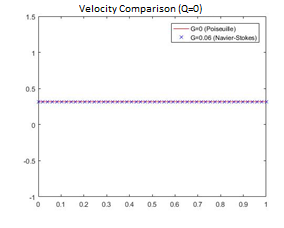
\includegraphics[width= 60mm]{Pressure_Gain_0}%
\qquad \qquad
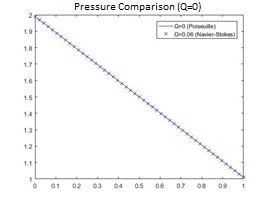
\includegraphics[width= 60mm]{Pressure_Gain_1}
\end{figure}
\begin{figure}[htbp]
\centering
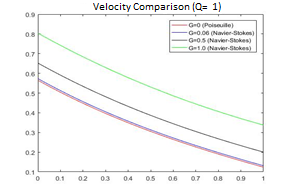
\includegraphics[width= 60mm]{Pressure_Gain_2}%
\qquad \qquad
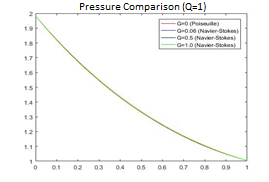
\includegraphics[width= 60mm]{Pressure_Gain_3}
\end{figure}
As we can see, if we solve both problems with dirichlet boundary conditions, with no exchange between the vessel and the porous medium ($Q=0$), there is no difference between the two solutions. Instead, if we solve it with non zero wall conductivity ($Q=1$), we have an increasing difference of the velocity solution as we increase the Dynamic Pressure Gain ($G>0$). In fact for a fixed pressure difference (due to the dirichlet boundary conditions) the transport term make the increase the velocity in channel.

\subsection{SingleBranch}

\begin{figure}[htbp]
\centering
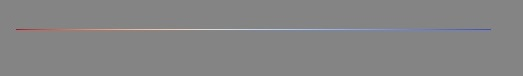
\includegraphics[width= 60mm]{SingleBranch_Rettilineo}%
\qquad \qquad
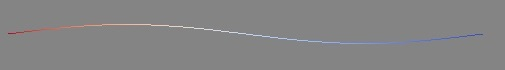
\includegraphics[width= 60mm]{SingleBranch_Curvo}
\end{figure}
n the second test case, we wanted to emphasize the how the geometry of the problem can affect the solution. So, we decided to test for the Pouiseuille code on a rectilinear vessel, and the Navier-Stokes on a sinusoidal one.  Both the geometries are tested with the same parameters and boundary conditions and on the sinusoidal branch we imposed zero Dynamic Pressure Gain, to avoid transport effects.

\begin{figure}[htbp]
\centering
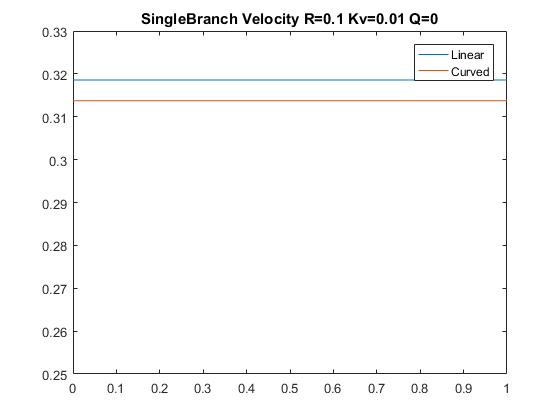
\includegraphics[width= 60mm]{SingleBranch_velocity_1}%
\qquad \qquad
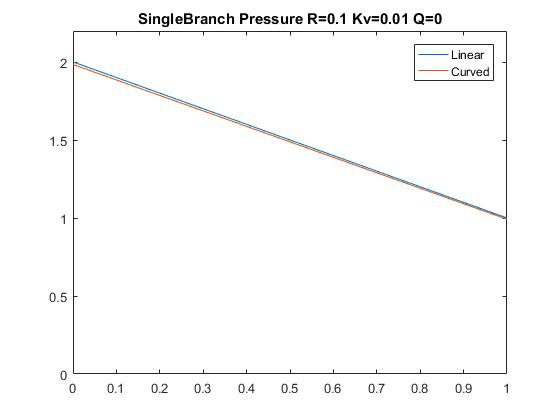
\includegraphics[width= 60mm]{SingleBranch_Pressure_1}
\end{figure}
\begin{figure}[htbp]
\centering
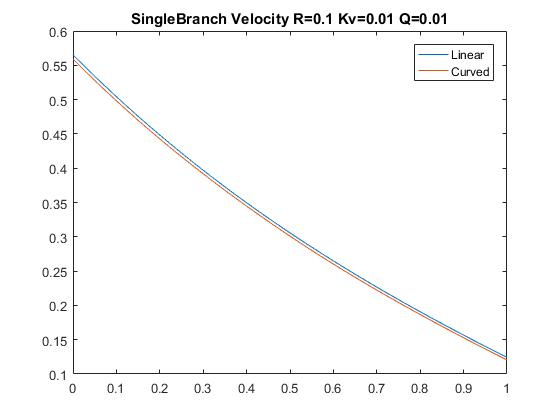
\includegraphics[width= 60mm]{SingleBranch_velocity_2}%
\qquad \qquad
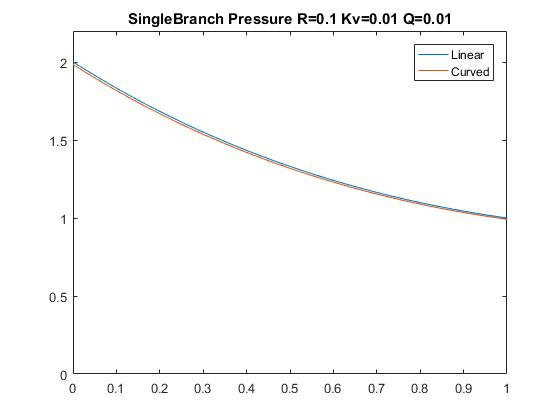
\includegraphics[width= 60mm]{SingleBranch_Pressure_2}
\end{figure}
In the this case we have a diminishing of velocity for the sinusoidal geometry for all choose of wall conductivity ($Q=0$ or $Q=0.01$). This effect is due to the fact that the mean effective conductivity for the rectilinear branch is higher than the curved one, and so for fixed pressure gradient (as we can see it's the same for both test) it allows an higher velocity. But for our simulation we choose the problem with a small effect due to the curvature ($\kappa R\ll1$) , so in the next example we tried to point it out ($\kappa R\sim1$).
\begin{figure}[ht]
\centering
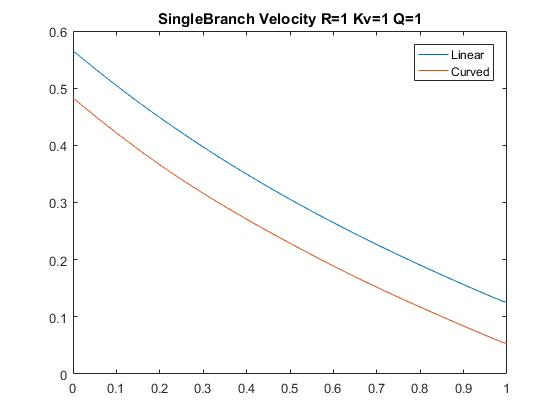
\includegraphics[width= 60mm]{SingleBranch_velocity_3}%
\qquad \qquad
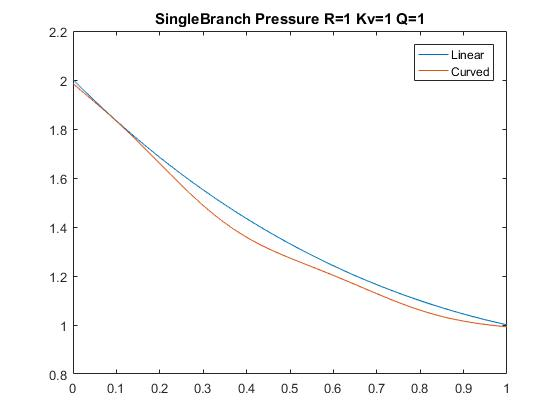
\includegraphics[width= 60mm]{SingleBranch_Pressure_3}
\end{figure}
\newpage
\begin{figure}[htbp]
\centering
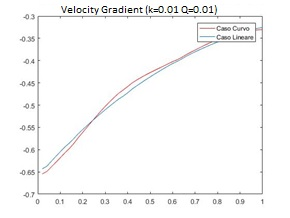
\includegraphics[width= 60mm]{SingleBranch_velocity_3_gradient}%
\qquad \qquad
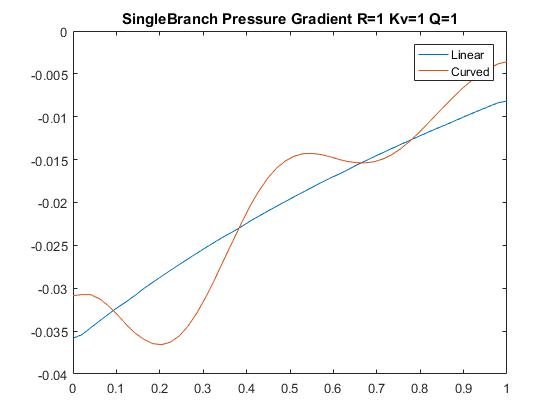
\includegraphics[width= 60mm]{SingleBranch_Pressure_3_gradient}
\end{figure}
From this plot we have an overview on how the curvature corrective coefficient really affect the solution. Here not only the velocity, but also the pressure has been influenced by the geometry. So in this simulation, we highlighted that the flow velocity decrease due to curvature effect and the pressure gradient follow the curvature trend.



\subsection{Bifurcartion}

\begin{figure}[htbp]
\centering
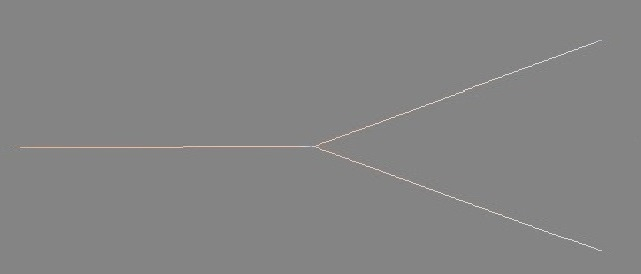
\includegraphics[width= 40mm]{Bifurcation_Rettilineo}%
\qquad \qquad
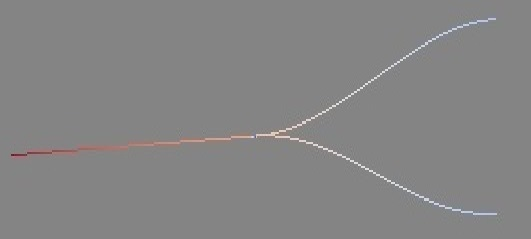
\includegraphics[width= 40mm]{Bifurcation_Curvo}%
\qquad \qquad
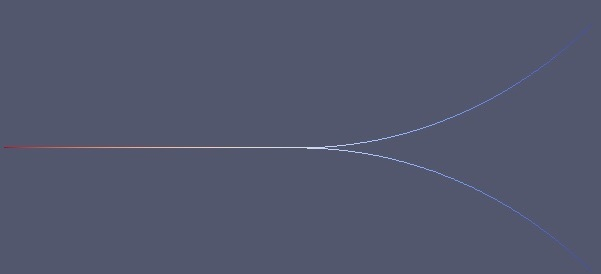
\includegraphics[width= 40mm]{Circular_Bifurcation}%
\end{figure}
The third test case is done on curved bifurcation with variable radius ($R=\{0.1 ,0.075,0.075\}$) for the Navier-Stokes model, and on a rectilinear bifurcation for the Pouiseuille one. In both simulations, we imposed for every branch the same conditions and the same parameters and for the Navier-Stokes case we impose a small effect of curvature ($\kappa R \ll1$). For curved test case were chosen two different profile, one sinusoidal and one circular.

\begin{figure}[htbp]
\centering
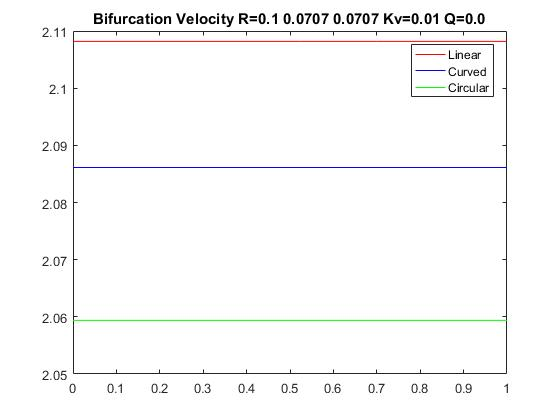
\includegraphics[width= 60mm]{Bifurcation_Velocity0}%
\qquad \qquad
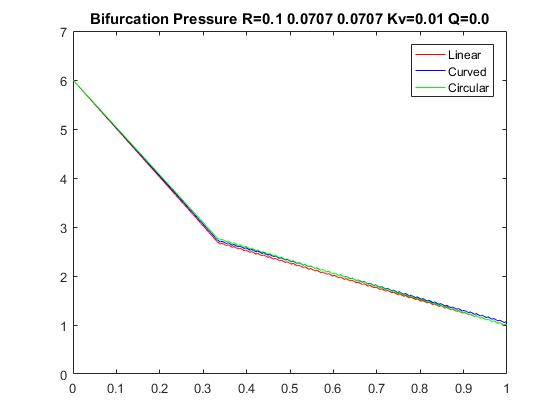
\includegraphics[width= 60mm]{Bifurcation_Pressure0}
\end{figure}
\newpage
\begin{figure}[htbp]
\centering
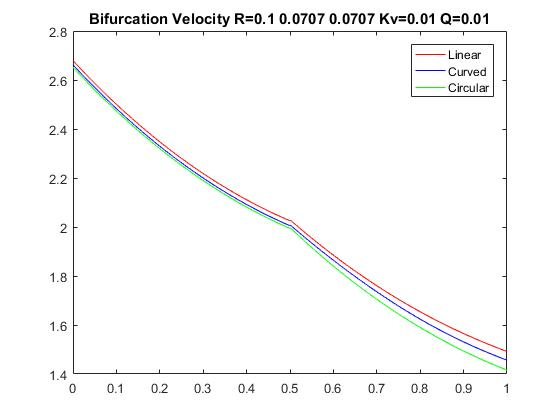
\includegraphics[width= 60mm]{Bifurcation_Velocity1}%
\qquad \qquad
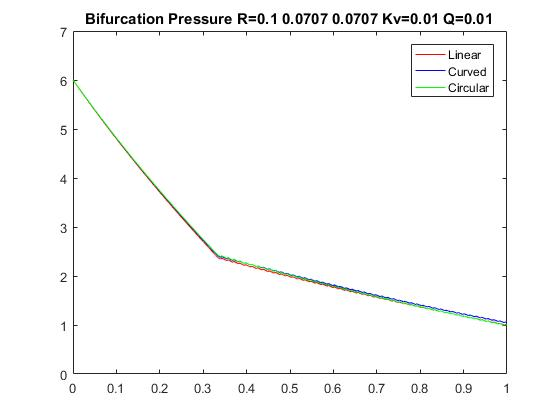
\includegraphics[width= 60mm]{Bifurcation_Pressure1}
\end{figure}
Through these plots we have strong disagreement between the solutions also for a low curvature effect. 
First of all, from the case with null wall permeability ($Q=0$),we have that the velocity decreases in the network with the increasing of the curvature effect. That is due, as for the SingleBranch, to geometric effect on the conductivity of the channel, which decrease in presence of curvature. To highlight this point we compare the sinusoidal and the circular test and we have lower velocity in the second one, because it has a constant and higher curvature, with respect to the first one, on the branches after the bifurcation. For the non zero wall permeability cases, we have almost the same result but, for presence of the curved geometry, the velocity decrease faster when we have a higher geometric effect.\\
For this kind of tests case, it is possible to find different velocity profiles before and after the junction, so the solution could have the presence of jump of velocity.\\
Let's derive how much this change of profile could affect our solutions. Due to the continuity condition in junctions, we have:
\begin{multline}
0= \sum_{i \in J_{in}} \int_{A_i} u_z^i dA - \sum_{j \in J_{out}} \int_{A_j} u^j_z dA = \\
 \sum_{i \in J_{in}}\overline{u}^i_z \int_{A_i} p_i(r,\theta) dA - \sum_{j \in J_{out}} \overline{u}^j_z \int_{A_j} p_j(r,\theta) dA 
\end{multline}
where $p_i$ is the velocity profile over the branch $i$. Now using the full velocity profile formula we have:
\begin{equation}
\int_{A_i} [p_i(r,\theta)] dA =\int_{A_i} [s(r)(1+\kappa_i^2r^2-2 \kappa_i r \cos \theta)] dA= \pi R_i^2+\pi \kappa_i R_i^4 \sigma
\end{equation}
with $\sigma =\frac{\gamma+2}{4(\gamma+2)}$ and $\gamma$ is the order of velocity profile.\\
Due to this we have:
\begin{multline}
0= \sum_{i \in J_{in}} \int_{A_i} u_z^i dA - \sum_{j \in J_{out}} \int_{A_j} u^j_z dA =\\
=(\sum_{i \in J_{in}} \overline{u}_z^i \pi R_i^2 - \sum_{j \in J_{out}}\overline{u}_z^j \pi R_j^2)+\sigma(\sum_{i \in J_{in}} \overline{u}_z^i \pi R_i^4 \kappa_i^2 - \sum_{j \in J_{out}}\overline{u}_z^j \pi R_j^4 \kappa_j^2)
\end{multline}
As we can see from this formula, with respect to the linear case we have an additive term which take care of this change of velocity profile and that could create jumps of velocity. But for low curvature effect, this term looks negligible with respect the linear one, as we can see from the circular case.

\newpage
\subsection{Rhombus}
\begin{figure}[htbp]
\centering
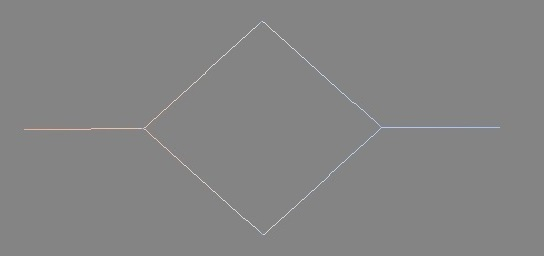
\includegraphics[width= 40mm]{Rombo_Rettilineo}%
\qquad \qquad
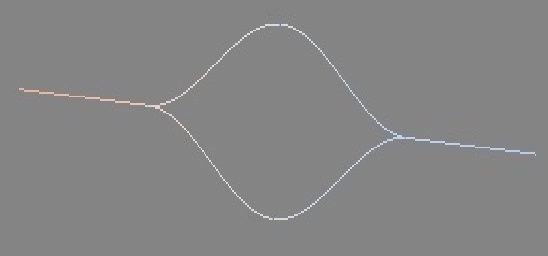
\includegraphics[width= 40mm]{Rombo_Curvo}%
\qquad \qquad
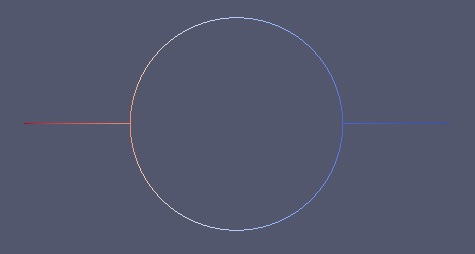
\includegraphics[width= 40mm]{Circular_rhombus}%
\end{figure}
r the last test case we decided to test the two solvers for a rhomboidal geometry, with a variable radius ($R=\{0.05,0.035, 0.035, 0.035,0.05\}$), zero Dynamic Pressure Gain ($G=0$) and low curvature effect ($\kappa R\ll1$).
\begin{figure}[htbp]
\centering
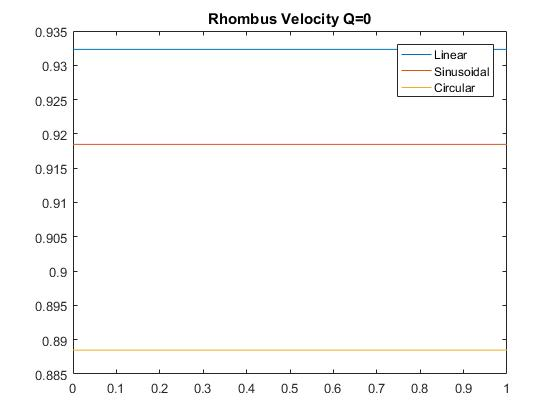
\includegraphics[width= 60mm]{Rombus_Velocity0}%
\qquad \qquad
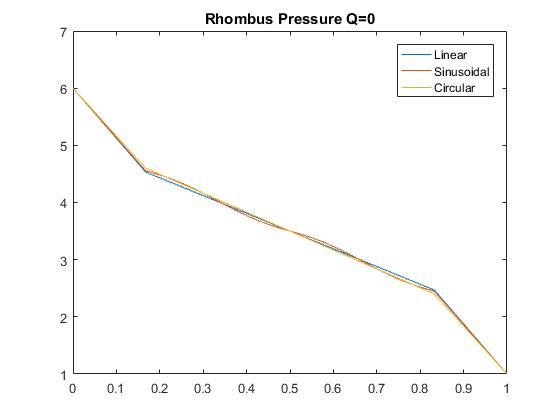
\includegraphics[width= 60mm]{Rombus_Pressure0}
\end{figure}
\begin{figure}[htbp]
\centering
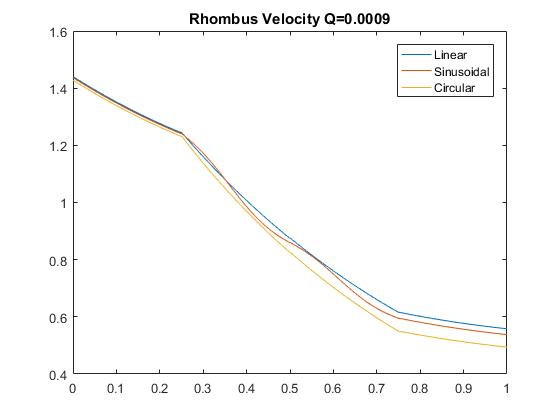
\includegraphics[width= 60mm]{Rombus_Velocity1}%
\qquad \qquad
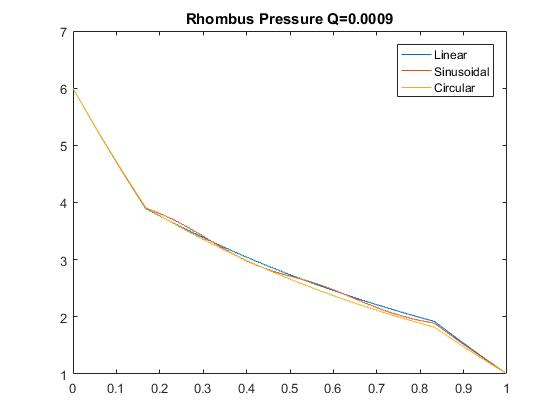
\includegraphics[width= 60mm]{Rombus_Pressure1}
\end{figure}

As for the previous test, we have that higher mean curvature implies less conductivity of channel. So for the curved networks, we have lower velocity, in the cases with zero wall permeability, and faster velocity decreasing in the branch with higher curvature, for the case with non zero wall permeability.

\subsection{Conclusion}
Thanks to our tests, we can conclude that for a rectilinear problem with very low Dynamic Pressure Gain, both the solvers reach almost the same solution.
Higher Dynamic Pressure Gain has the effect to increase the velocity in the vessel for a constant pressure gradient.
In the end, in presence of curved geometries we have a general reduction of the conductivity of the vessel, which can affect all the network in different ways. In the Siglebranch, there is a reduction of the flow velocity due to the lower conductivity. For a more complex geometry, we have a general reduction of the flow velocity in the network, due to the reduction of the mean conductivity, and for diffusing vessel, we have a faster decreasing of velocity in the curved branches with respect to the rectilinear ones.

\newpage
\chapter{C++ code}
The latest stable release of the code is available at the following link:
\begin{equation*}
https://github.com/lformaggia/model3D1D
\end{equation*}
Let us briefly review the main achievements. The code is divided into three main section: MixedFormulation, CurvedFormulation and GraphGenerator. The first one is the code developed by Domenico Notaro, which contain the solver for simple linear geometry based on Pouiseuille Flow assumption, using getFem++ library. The second one is code for the resolution of microcirculation problems for a more generic network geometry, that we modeled in the previous sections. The last one is code which use the library BGLgeom of M. Tantardini and I. Speranza in order to produce a simple tool for generate a the network.


\section{CurvedFormulation}
For the microcirculation part, we decide to use the same structure implemented by D. Notaro in his code and to do real modification only on those structures which doesn't adapt to the generic geometry, and for that we make great use of the library $libproblem3d1d.a$.\\
The first real modification is on the declaration of the main structure representing the 3D/1D problem, in an appropriate header($c\_\-problem3d1d.hpp$), and his definition in a source file ($c\_\-problem3d1d.cpp$). Thanks to the similarities with the Poiseuille model, for this structure is used a class derived from the class $problem3d1d$ implemented in the MixedFormulation. \\
As for the MixedFormulation we keep inside the main class all the attributes who identify an instance of the problem, such as the meshes, finite elements methods, boundary condition and so on. On the other hand, external attributes such as the user-defined descriptors of the algorithm ($c\_\-desc3d1d.hpp$) , the physical parameters ($c\_\- param3d1d.hpp$) have been moved to proper header files.
Furthermore, following the two main design principle of OOP, namely $encapsulation$ and $information$ $hiding$, we define a simple interface between the computational model and the user: the whole internal structure has \textbf{ private} scope while public accessors are eventually provided to inspect the attributes.\\

\newpage
\subsection{c\_\-problem3d1d}
{\fontfamily{qcr}\selectfont
//! Main class defining the coupled 3D/1D fluid curved problem\\

\textbf{class c\_\-problem3d1d: public problem3d1d \{}\\
//! Initialize the problem\\
/*!\\
\tab 1.Read the .param filename from standard input\\
\tab 2.Import problem descriptors (file path, GetFEM types,...)\\
\tab 3.Import mesh for tissue (3D) and vessel network (1D)\\
\tab 4.Set finite elements and integration methods\\
\tab 5.Build problem parameters\\
\tab 6.Build the list of tissue boundary data\\
\tab 7.Build the list of vessel boundary (and junction) data\\
*/	 \\
\textbf{init(int argc, char *argv[]);}\\
//! Assemble the problem\\
/*!\\
\tab 1. Initialize problem matrices and vectors\\
\tab 2. Build the monolithic matrix AM\\
\tab 3. Build the monolithic rhs FM\\
*/\\
\textbf{void assembly(void);}\\
//! Solve the problem\\
/*!	\\
\tab Solve iteratively the monolithic system at each iteration until stop conditions are reached\\
*/\\
\textbf{bool solve(void);}\\
/*!\\
\tab Merge arterial and venous networks.\\
\tab Solve iteratively the monolithic system\\
*/\\
\textbf{friend bool merge\_\-and\_\-solve(c\_\-problem3d1d \& Pa, c\_\-problem3d1d \& Pv);}\\
//! Export results into vtk files\\
/*!\\
\tab Export solutions $ U_t , P_t , U_v , P_v $ from the monolithic array UM\\
*/\\
\textbf{void export\_\-vtk(const string \& suff= "");}\\
//! Compute mean tissue pressure\\
\textbf{inline scalar\_\-type mean\_\-pt(void) }\{\\ \tab return asm\_\-mean(mf\_\-pt, mimt,\\ \tab \tab gmm::sub\_\-vector(UM,gmm::sub\_\-interval(dof.Ut(),dof.Pt())));\\ \} \\
//! Compute mean vessel pressure\\
\textbf{inline scalar\_\-type mean\_\-pv(void)}\{\\ 
\tab return asm\_\-mean(mf\_\-pv, mimv,
\\ \tab \tab gmm::sub\_\-vector(UM,gmm::sub\_\-interval(dof.Ut()+dof.Pt()+dof.Uv(),dof.Pt())));\\ \} \\
//! Compute mean vessel velocity\\
\textbf{inline scalar\_\-type mean\_\-uv(void)}\{\\
\tab size\_\-type dofi=0;\\
\tab size\_\-type shift=dof.Ut()+dof.Pt();\\
\tab scalar\_\-type mean=0.0;\\
\tab for(size\_\-type branch=0; branch<mf\_\-Uvi.size(); branch++)\{\\
\tab \tab shift+=dofi;\\
\tab \tab dofi=mf\_\-Uvi[branch].nb\_\-dof();\\
\tab \tab mean+=asm\_\-mean(mf\_\-Uvi[branch],mimv,gmm::sub\_\-vector(UM,\\
\tab \tab \tab gmm::sub\_\-interval(shift,dofi)));\\
\tab \}\\
\tab return mean/mf\_\-Uvi.size();\\
\}\\
//!Compute the dynamic pressure gain\\
\textbf{inline scalar\_\-type G(void)}\{\\
\tab return c\_\-param.G(0);\\
\}\\
//! Compute total flow rate (network to tissue) - pressure\\
\textbf{inline scalar\_\-type flow\_\-rate(void)}\{ return TFR; \}\\ \\
protected:\\ \\
//! Algorithm description strings of curved model\\
\textbf{c\_\-desc3d1d c\_\-descr;}\\
//! Physical parameters (dimensionless) for curved model\\
\textbf{c\_\-param3d1d c\_\-param;}\\
//! Velocity in the vessel at a previous iteration\\
\textbf{vector\_\-type Uv\_\-old;}\\
//! Non linear matrix for transport term\\
\textbf{sparse\_\-matrix\_\-type NLMvv;}\\
//! Non linear matrix for Junction transport effect\\
\textbf{sparse\_\-matrix\_\-type NLJvv;}\\
//! Full non linear matrix
\textbf{sparse\_\-matrix\_\-type NL;}\\
//! Non linear RHS effect (used only in Newton Method)\\
\textbf{vector\_\-type NLF;}\\
//! Monolithic matrix with both linear and non linear term\\
\textbf{sparse\_\-matrix CM;}\\
//! Monolithic RHS with both linear and non linear term\\
\textbf{vector\_\-type CFM;}\\ \\
//! Import algorithm specifications\\
\textbf{void import\_\-data(void);}\\
//! Import mesh for tissue (3D) and vessel (1D)\\
\textbf{void build\_\-mesh(void);}\\
//! Set finite elements methods and integration methods\\
\textbf{void set\_\-im\_\-and\_\-fem(void);}\\
//! Build problem parameters\\
\textbf{void build\_\-param(void);}\\
//! Build the list of tissue boundary data\\
	/*!	Face numbering:\\
	\tab 0 : \{x = 0 \}  "back"\\
	\tab 1 : \{x = Lx\}  "front"\\
	\tab  2 : \{y = 0 \}  "left"\\
	\tab  3 : \{y = Ly\}  "right"\\
	\tab  4 : \{z = 0 \}  "bottom"\\
	\tab  5 : \{z = Lz\}  "top"\\
	*/\\
\textbf{void build\_\-tissue\_\-boundary(void);}\\
//!Build the list of vessel boundary (and junctions) data\\
\textbf{void build\_\-vessel\_\-boundary(void);}\\
//! Build the monolithic matrix AM by blocks\\
\textbf{void assembly\_\-mat(void);}\\
//! Build the monolithic rhs FM by blocks\\
\textbf{void assembly\_\-rhs(void);}\\
//! Assemble RHS source term for stand-alone tissue problem\\
\textbf{void assembly\_\-tissue\_\-test\_\-rhs(void);}\\
//! Build non linear matrix NL\\
\textbf{assembly\_\-nonlineat\_\-mat(void);}\\
//! Solve the monolithic system for a given iteration\\ //! of the fixed point method\\
\textbf{bool solve\_\-pass(size\_\-pass iter=0);}\\
\}; /*end of class c\_\-problem3d1d
}\\ \\ -------------------------------------------------------------------------------------------------------------------------------------\\
Moreover many other elements (matrix and parameters) are directly imported by the "$problem3d1d$" class.\\
This approach allows to build the most generic tool that is at the same time the easiest possible for incoming "non developing" users and, at the same time, to safeguard the developer from the risks of altering the implementation. In the end, the only methods that remain \textbf{public} define exactly what one needs to do in a main file, that is to (I) declare a new instance of the problem, (II) set problem's parameters and initialize the problem, (III) assemble the linear system, (IV) solve it and finally (V) save results for post-processing.
\\ -------------------------------------------------------------------------------------------------------------------------------------\\ \\

{\fontfamily{qcr}\selectfont
// Declare a new problem\\
\textbf{getfem::c\_\-problem3d1d p;}\\
// Initialize the problem\\
\textbf{p.init(argc,argv);}\\
// Build the monolithic system\\
\textbf{p.assembly();}\\
// Solve the problem\\
\textbf{if(!p.solve()) GMM\_\-ASSERT1(false,"solve procedure has failed");}\\
// Save results in .vtk format\\
\textbf{p.export\_\-vtk();}\\
// Display some global results: mean pressures,  total flow rate\\
\textbf{std::cout<<"} Pt average = " \textbf{<< p.mean\_\-pt()<< std::endl;}\\
\textbf{std::cout<<"} Pv average  =" \textbf{<<p.mean\_\-pv()<<std::endl;}\\
\textbf{std::cout<<"} Uv average  =" \textbf{<<p.mean\_\-uv()<<std::endl;}\\
\textbf{std::cout<<"} Network-to-Tissue TFR =" \textbf{<<p-flow\_\-rate()<<std::endl;}\\
...
}
\newpage -----------------------------------------------------------------------------------------------------------------------------------\\
After these manipulations the package has the following hierarchical structure:\\
\tab {\fontfamily{qcr}\selectfont doc/}: Code documentation (to be generate)\\
\tab {\fontfamily{qcr}\selectfont include/}: General header files\\
\tab {\fontfamily{qcr}\selectfont lib/}: Main library (to be generate)\\
\tab{\fontfamily{qcr}\selectfont src/}: Example sources\\
\tab \tab {\fontfamily{qcr}\selectfont 1\_\-LinearSingleBranch/} Solve the linear SingleBranch\\
\tab \tab {\fontfamily{qcr}\selectfont 2\_\-CurvedSingleBranch/} Solve the curved SingleBranch\\
\tab \tab {\fontfamily{qcr}\selectfont 3\_\-LinearBifurcation/} Solve the linear Bifurcation\\
\tab \tab {\fontfamily{qcr}\selectfont 4\_\-CurvedBifurcation/} Solve the curved Bifurcation \\
\tab \tab {\fontfamily{qcr}\selectfont 5\_\-LinearRombus/} Solve the linear Rhombus\\
\tab \tab {\fontfamily{qcr}\selectfont 6\_\-CurvedRombus/} Solve the curved Rhombus \\
\tab {\fontfamily{qcr}\selectfont Doxyfile/}: Instruction to build the code documentation\\
\tab {\fontfamily{qcr}\selectfont Makefile/}: Instruction to install the whole project\\
It can be seen that the provided examples follows exactly the benchmarks provided in Chapter 4. The identical structure has been preserved in almost all subdirectories, namely:\\
\tab {\fontfamily{qcr}\selectfont vtk/}: Output in vtk format\\
\tab {\fontfamily{qcr}\selectfont input.param/}: List of user-defined parameters\\
\tab {\fontfamily{qcr}\selectfont main.cpp/}: Main program\\
\tab {\fontfamily{qcr}\selectfont Makefile/}: Instruction to install the example\\
\tab {\fontfamily{qcr}\selectfont network.pts/}: File of points of the vessel network\\
\tab {\fontfamily{qcr}\selectfont network\_\-geometry.pts/}: File of geometric parameters\\

\subsection{Mesh and Parameters}
Particular attentions is necessary when we read the input file for the mesh1d and the parameters. In fact the difference from the linear problem (MixedFormulation) we need to recive as input not only the point of mesh but also the value of the curved parameters in that, and subsequently we need to interpolate that parameter value on the proper mesh\_\-fem. The curvature value is given in each node of the mesh, so for it we used $P(1,1)$ (polynomial interpolation 1d functions of degree 1) finite elements. Instead the tangent versor is computed as constant over each element of the mesh, so for it we used $P(0,1)$ finite elements. 
For that in the $c\_\-mesh1d.hpp$ header are implemented the function able to manage on it. 
{\fontfamily{qcr}\selectfont
/*!
 Create the edge sequence and build the related 1D mesh. \\
  The input stream ist is used to read a file with the following format (gambit-like): \\
\\
\tab		BEGIN\_\-LIST\\
\tab		BEGIN\_\-ARC \\
\tab		BC KEYWA [VALUES] \\
\tab		BC KEYWB [VALUES]\\
\tab		 106       0.4421      -1.6311       2.5101		start\\
\tab		 107       0.4421      -1.6311       7.5101		end  \\
\tab		 108       0.3546      -1.6524       2.5539		point\\
\tab		 109       0.2621      -1.6695       2.5880		point\\
\tab		... \\
\tab		END\_\-ARC \\
\tab		... \\
\tab		BEGIN\_\-ARC  \\
\tab		... \\
\tab		END\_\-ARC \\
\tab		... \\
\tab		END\_\-LIST \\

  1. The list of points of the IS ordered as follows:\\
\tab     - first we have the coordinates of TWO ENDS (A,B) (i.e. A=start and B=end)\\
\tab     - then we have all the remaining nodes of the arc, from A to B\\
  2. If a node is shared by more arcs, the arcs will be CONNECTED in the resulting 1D mesh.\\
  3. BC KEYWA [VALUES] and BC KEYWB [VALUES] are keywords/values related to boundary conditions\\
     to be imposed at nodes A, B. Each KEYW [VALUES] entry can be one of the following: \\
\tab     - BC DIR 1.1\\
\tab     - BC MIX \\
\tab     - BC INT \\
     Correspondingly, each node will be marked with the associated boundary condition, that are:\\
\tab     - Dirichlet node (pressure = 1.1)\\
\tab     - Mixed     node (flux = coef*(pressure - p0))\\
\tab     - Internal  node\\
     At this stage, this is only meant to assign such BC labels to each node.\\
     If one end is INTERNAL, the corresponding BC will be ignored \\
     (for clarity, please write the INT keyword).     \\
\\
\\
     The input stream istc is used to read a file with the following format (gambit-like): \\
\\
\tab		BEGIN\_\-LIST\\
\tab		BEGIN\_\-ARC \\
\tab		BC KEYWA [VALUES] \\
\tab		BC KEYWB [VALUES]\\
\tab		 106       0.4421      -1.6311       2.5101		0.1221		0.3454		0.2943		0.7561 start\\
\tab		 107       0.4421      -1.6311       7.5101		0.1221		0.3454		0.2943		0.7561 end  \\
\tab		 108       0.3546      -1.6524       2.5539		0.2235		0.2541		0.3012		0.7214 point\\
\tab		 109       0.2621      -1.6695       2.5880		0.2173		0.2497		0.2886		0.7493 point\\
\tab		... \\
\tab		END\_\-ARC \\
\tab		... \\
\tab		BEGIN\_\-ARC  \\
\tab		... \\
\tab		END\_\-ARC \\
\tab		... \\
\tab		END\_\-LIST \\
\\
  1. The list of points of the IS ordered as follows:\\
\tab     - first we have the parameters for the TWO ENDS coordinate (A,B) (i.e. A=start and B=end)\\
\tab     - then we have all the remaining parameters for the nodes of the arc, from A to B\\
  2. If a node is shared by more arcs, the arcs will be CONNECTED in the resulting 1D mesh.\\
  3. BC KEYWA [VALUES] and BC KEYWB [VALUES] are keywords/values related to boundary conditions\\
     to be imposed at nodes A, B. For this kind of problem is not required any boundary condition\\
     fot the curved parameters, because all the BC are imposed with the mesh file input. If the \\
     reader would find any BC, it will simply avoid to read it.\\
*/\\ \\
/*!\\
\tab	Import the network points and the curved paremeters from the file pts and build the
	mesh.\\
 */\\
//! It also build vessel mesh regions (\#=0 for branch 0, \#=1 for branch 1, ...).\\
\textbf{
template<typename VEC\_\-SIZE, typename PARAM>\\
void import\_\-pts\_\-file}(\\
\tab		std::istream \& ist, \\
\tab		std::istream \& istc,\\
\tab		getfem::mesh \& mh1D, \\
\tab		std::vector<getfem::node> \&  BCList,\\
\tab		VEC\_\-SIZE \& Nn,\\
\tab		const std::string \& MESH\_\-TYPE,\\
\tab		PARAM \& param\\
\tab		) \\
\\
/*!\\
\tab	Reassemble the curved parameters on the data finite elements.\\
\tab	The parameters are given in the coordinates of the mesh, so it is\\
\tab	assumed that the parameters are imported using polynomial of degree 1\\
\tab 	for curvature and polynomial of degree 0 for tangent versor.\\
*/\\
\textbf{
template<typename VEC, typename VEC\_\-FEM>
void rasm\_\-curve\_\-parameter}(\\
\tab		VEC\_\-FEM \& mf\_\-Coefi,\\
\tab		VEC \& Curv,\\
\tab		VEC \& lx,\\
\tab		VEC \& ly,\\
\tab		VEC \& lz\\
\tab	)\\

\{\\
\tab	VEC Curv\_\-temp=Curv;\\
\tab	VEC lx\_\-temp=lx;\\
\tab	VEC ly\_\-temp=ly;\\
\tab	VEC lz\_\-temp=lz;\\
\tab	size\_\-type Nb=Curv\_\-temp.size(); //Number of branch\\
\tab	size\_\-type Ni=0; //Number of dof of the coefficient mesh at branch i\\
\tab    //Fem descriptor for curvature\\
\tab	pfem fd\_\-curv = fem\_\-descriptor("FEM\_\-PK(1,1)");\\
\tab   //Fem descriptor for tangent versor\\
\tab	pfem fd\_\-tgv  = fem\_\-descriptor("FEM\_\-PK(1,0)"); \\
\tab	scalar\_\-type ct;\\
\tab	for(size\_\-type b=0; b<Nb;++b)\{\\
\tab\tab	Ni=Curv\_\-temp[b].size();\\
	\\
\tab\tab		//Reodering the value of the parameters\\
\tab\tab		ct=Curv[b][1];\\
\tab\tab		   //Shifting all elements\\
\tab\tab		for(size\_\-type i=2; i<Curv\_\-temp[b].size(); i++)\{\\
\tab\tab\tab			Curv\_\-temp[b][i-1]=Curv[b][i];\\
\tab\tab		\}\\
\tab\tab		Curv\_\-temp[b].back()=ct;\\
\\
\tab\tab		//Adapting parameters to tbe finite element interpolation\\
\tab\tab		Ni=mf\_\-Coefi[b].nb\_\-dof();\\
\tab\tab		Curv[b].resize(Ni); gmm::clear(Curv[b]);\\
\tab\tab		 lx[b].resize(Ni);  gmm::clear(lx[b]);\\
\tab\tab		 ly[b].resize(Ni);  gmm::clear(lx[b]);\\
\tab\tab		 lz[b].resize(Ni);  gmm::clear(lx[b]);\\
\\		
\tab\tab		//Generating the P1 finite element for curvature\\
\tab\tab		getfem::mesh\_\-fem mf\_\-curv(mf\_\-Coefi[b].linked\_\-mesh());\\
\tab\tab		mf\_\-curv.set\_\-finite\_\-element(mf\_\-Coefi[b].linked\_\-mesh().region(b).index(),\\ \tab \tab \tab \tab \tab \tab \tab \tab \tab fd\_\-curv);\\
\\
\tab\tab		//Generating the P0 finite element for tangent versor\\
\tab\tab		getfem::mesh\_\-fem mf\_\-tgv(mf\_\-Coefi[b].linked\_\-mesh());\\
\tab\tab		mf\_\-tgv.set\_\-finite\_\-element(mf\_\-Coefi[b].linked\_\-mesh().region(b).index(), \\ \tab \tab \tab \tab \tab \tab \tab \tab \tab fd\_\-tgv);\\
\\
\tab\tab		//Interpolating v curvature on a different mesh fem \\
\tab\tab		gmm::row\_\-matrix<vector\_\-type> M\_\-curv(mf\_\-Coefi[b].nb\_\-dof(),\\ \tab \tab \tab \tab \tab \tab \tab \tab \tab mf\_\-curv.nb\_\-dof());\\
\tab\tab		getfem::interpolation(mf\_\-curv,mf\_\-Coefi[b],M\_\-curv);\\
\tab\tab		gmm::mult(M\_\-curv,Curv\_\-temp[b],Curv[b]);\\
\\

\tab\tab		//Interpolating v curvature on a different mesh fem \\
\tab\tab		gmm::row\_\-matrix<vector\_\-type> M\_\-tgv(mf\_\-Coefi[b].nb\_\-dof(),\\ \tab \tab \tab \tab \tab \tab \tab \tab \tab mf\_\-tgv.nb\_\-dof());\\
\tab\tab		getfem::interpolation(mf\_\-tgv,mf\_\-Coefi[b],M\_\-tgv);\\
\tab\tab		gmm::mult(M\_\-tgv,lx\_\-temp[b],lx[b]);\\
\tab\tab		gmm::mult(M\_\-tgv,ly\_\-temp[b],ly[b]);\\
\tab\tab		gmm::mult(M\_\-tgv,lz\_\-temp[b],lz[b]);\\
\\
\tab\tab		gmm::clear(M\_\-tgv);\tab gmm::clear(M\_\-curv);\\
\tab	\}
\}


}
\subsection{Assembling}
For the system derivation we used some auxiliary functions, defined in the proper header ($assembling1d3d.hpp$, $assembling1d.hpp$, $assembling3d.hpp$, $c\_\-assembling1d.hpp$). Many functions for the matrices implementation are already done in the a MixedFormulation, with some change of parameters, but the nonlinear part still needed to be implemented.\\

{\fontfamily{qcr}\selectfont
//! Build the advective non linear matrix for the 1D Navier-Stokes curved \\ \tab \tab problem,\\
//! $ NLM = \int_{\Lambda} c~u~uold~\nabla v \cdot \mathbf{\lambda}\,~ds $\\
/*!\\
\tab	NLM  \tab \,     Computed non linear matrix term\\
\tab	 mim   \tab \, The integration method to be used\\
\tab	mf\_\-u \tab     The finite element method for the velocity $ \mathbf{u} $\\
\tab	mf\_\-data \,    The finite element method for the tangent versor on $ \Lambda $\\
\tab	coef   \tab   The coefficient for NLM\\
\tab	lambdax \,   First cartesian component of the tangent versor  $ \mathbf{\lambda} $\\
\tab	lambday \,   Second cartesian component of the tangent versor $ \mathbf{\lambda} $\\
\tab	lambdaz \,   Third cartesian component of the tangent versor $ \mathbf{\lambda}$\\
\tab	u\_\-old \, \,      The velocity at the previous iteration\\
\tab	rg    \tab  \,    The region where to integrate\\
 */\\
\textbf{template<typename MAT, typename VEC>\\
void asm\_\-network\_\-nonlinear}(\\
\tab	MAT \& NLM,\\
\tab	 const mesh\_\-im \& mim,\\
\tab	 const mesh\_\-fem \& mf\_\-u,\\
\tab	 const mesh\_\-fem \& mf\_\-data,\\
\tab	 const VEC \& coef,\\
\tab	 const VEC \& lambdax,\\ \tab const VEC \& lambday,\\ \tab  const VEC \& lambdaz,\\
\tab	 const VEC \& u\_\-old,\\
\tab	 const mesh\_\-region \& rg = mesh\_\-region::all\_\-convexes()\\
\tab	 ) 		\\
\{\\
\tab	GMM\_\-ASSERT1(mf\_\-u.get\_\-qdim() == 1,"invalid data mesh fem (Qdim=1 required)");\\
\tab	// Build the local matrix for the non linear term NLMvvi\\
\tab	generic\_\-assembly \\
\tab \tab	assem("l1=data\$1(\#2); l2=data\$2(\#2); l3=data\$3(\#2);\\\tab\tab\tab\tab u=data\$4(\#1); c=data\$5(\#2);"\\
\tab\tab \tab		  "t=comp(Base(\#1).Base(\#1).Grad(\#1).Base(\#2).Base(\#2));"\\
\tab\tab\tab		  "M\$1(\#1,\#1)+=t(j,:,:,1,m,k).l1(m).u(j).c(k)+\\ \tab\tab \tab\tab t(j,:,:,2,m,k).l2(m).u(j).c(k)+ \\ \tab\tab \tab\tab t(j,:,:,3,m,k).l3(m).u(j).c(k);");\\
\tab	assem.push\_\-mi(mim);\\
\tab	assem.push\_\-mf(mf\_\-u);\\
\tab	assem.push\_\-mf(mf\_\-data);\\
\tab	assem.push\_\-data(lambdax);\\
\tab	assem.push\_\-data(lambday);\\
\tab	assem.push\_\-data(lambdaz);\\
\tab	assem.push\_\-data(u\_\-old);\\
\tab	assem.push\_\-data(coef);\\
\tab	assem.push\_\-mat(NLM);\\
\tab	assem.assembly(rg);\\
\}

}
\subsection{The library c\_\-problem3d1d}
In light of the final release of the code, we collect all routines external functions and variables defining out coupled 3D/1D curved problem,to build a $static$ library. This is hence resolved in a caller at compile-time and copied into a target application by a compiler, linker, or binder, producing an object file and a stand-alone executable.\\
The library {\fontfamily{qcr}\selectfont libc\_\-problem3d1d.a} can be automatically built using the provided Makefile and it is indeed adopted for all provided examples. It is built from following headers and sources:\\ \\
\tab {\fontfamily{qcr}\selectfont c\_\-assembling1d.hpp}: Miscellanous non linear assembly routine for 1D network problem\\
\tab {\fontfamily{qcr}\selectfont c\_\-descr3d1d.hpp}Definition f the aux class for algorithm curved description strings\\
\tab {\fontfamily{qcr}\selectfont c\_\-mesh1d.hpp}: Miscellanous handlers for 1D curved network mesh\\
\tab {\fontfamily{qcr}\selectfont c\_\-param3d1d.hpp} Definition of the aux class for physical parameters\\
\tab {\fontfamily{qcr}\selectfont c\_\-problem3d1d.cpp} Declaration of the main class for 3D/1D coupled curved problem\\
\tab {\fontfamily{qcr}\selectfont c\_\-problem3d1d.hpp} Definition of the main class for 3D/1D coupled curved problem\\
Remember that this library must be used with the library $libproblem3d1d.a$\\
See the README file for installation instructions.

\section{GraphGenerator}
The GraphGenerator gives as simple tool in order to easily generate complex networks with curved geometry. For the implementation is used the $ BGLgeom$ library of M. Tantardini and I. Speranza, which is able manage and create complex network geometry.\\
To easily manage this problem we split it in three part: read the graph control points,  generate the graph, generate two pts files containing the mesh and curved parameters on the points of the mesh.\\

\subsection{Implementation}
The first part is done through the class {\fontfamily{qcr}\selectfont B\_\-reader\_\-netdiff} (in the header $spline_reader.hpp$) derived from the parent class {\fontfamily{qcr}\selectfont BGLgeom::ASCII\_\-reader}. This class is able to read any ASCII file and to return the parameters needed to create the curved geometry.\\
The  ASCII Input file has to be of the following format:\\
\tab		Each branch is written in the same format and consecutively to the previous one.\\
\tab		They need:\\
\tab\tab		1) Boundaries conditions for the source and the target point.\\
\tab\tab		2) The number of point insert for the branch.\\
\tab\tab		3) The size of the mesh we want in the output for that branch.\\
\tab\tab		4) The source of the branch.\\
\tab\tab		5) The target of the branch.\\
\tab\tab		6) All the other nodes in the correct order.\\
\\ {\fontfamily{qcr}\selectfont
\tab	Example:\\
\\	
\tab		DIR 1.0 INT 0.0\tab 		(first branch)\\
\tab		3 100					\\
\tab		0.0 0.0 0.0\tab				(source node)\\
\tab		1.0 1.0 1.0\tab				(target node)\\
\tab		0.5 0.5 0.5\tab				(internal node)\\
\tab		INT 0.0 DIR 2.0\tab 		(second branch)\\
\tab		5 50\\
\tab		1.0 1.0 1.0\\
\tab		3.0 3.0 3.0\\
\tab		1.5 1.6 1.5\\
\tab		2.0 2.0 2.0\\
\tab		2.4 2.3 2.4\\
\\
}

The last two parts are implemented in the function  {\fontfamily{qcr}\selectfont curved\_\-network\_\-reader} (whose definition is in the header $curved\_\-network\_\-reader.hpp$). This function require as input the name and location of the {\fontfamily{qcr}\selectfont input.param} file, in which are specified the descriptors strings needed for the generation of the network.\\
In this function, each branch is read one for time and after that, through the  class  {\fontfamily{qcr}\selectfont BGLgeom::bspline\_\-geometry}, it is constructed the branch using the $b\_\-spline$ $interpolation$ $method$ or $b\_\-spline$ $approximation$ $method$ and  is generate a uniform mesh on it, whose size is given in the input file.\\
The output part is already implemented in the  {\fontfamily{qcr}\selectfont BGLgeom} library and only require the name of the output pts file.\\
This is done in this form in order to give a simple tool to the user.\\	
\\ -------------------------------------------------------------------------------------------------------------------------------------\\ 
{\fontfamily{qcr}\selectfont 
int main(int argc, char *argv[])\{\\
\tab //Reading, constructing and exporting the network\\
\tab curved\_\-network\_\-reader(argc, argv);\\
\tab return 0;\\
\}
}
\\ -------------------------------------------------------------------------------------------------------------------------------------\\ \\
And in the {\fontfamily{qcr}\selectfont input.param} file is only needed to be specify three parameters: {\fontfamily{qcr}\selectfont INPUT\_\-ASCII="./ascii\_\-file"} for the input ASCII file name and location, {\fontfamily{qcr}\selectfont  INTERP=1} in order to use $b\_\-spline$ $interpolation$ $method$ for the branch construction, and {\fontfamily{qcr}\selectfont OUTPUT\_\-PTS="./network.pts"} for the output pts file name and location.

\subsection{The library graphgenerator}
As for the previous part, all routines are collected to build a $static$ library {\fontfamily{qcr}\selectfont libgraphgenerator.a}. That is automatically done by the Makefile and it is indeed adopted for the provided example. It is built from the following headers and source:\\
\tab {\fontfamily{qcr}\selectfont spline\_\-reader.hpp}: Definition of reader class for ASCII files\\
\tab {\fontfamily{qcr}\selectfont curved\_\-network\_\-reader.hpp}: Definition of main function for the generation of the network\\
\tab {\fontfamily{qcr}\selectfont curved\_\-network\_\-reader.cpp}: Declaration of main function for the generation of the network\\
Remember that this library must be used with the library $libBGLgeom.a$.\\
See the README file for installation instructions.


\begin{thebibliography}{9}

\bibitem{lamport94}
  D. Notaro,
  \emph{Mixed Finite Element Methods for Coupled 3D/1D Fluid Problem},
  Politecnico di Milano, Italy,
  2015 .

\bibitem{lamport94}
  L. Formaggia and A. Veneziani,
  \emph{Reduced and multiscale models for the human cardiovascular system},
  MOX, Mathematics Department "F. Brioschi",
  Politecnico di Milano, Italy,
  2003 .

\bibitem{lamport94}
  D. Lamponi,
  \emph{One dimensional and multiscale models for blood flow circulation},
  Ecole Polytechnique Federale de Lausanne, 
 2004 .

\bibitem{lamport94}
  T. Shifrin,
  \emph{Differential Geometry: A First Course in Curves and Surfaces},
  University of Georgia, 
 2016.


\bibitem{lamport94}
  L. Bergamaschi, S. Mantica and G. Manzini,
  \emph{A mixed finite element-finite volume formulation of the black-oil model},
 SIAM Journal on Scientific Computing, 
 20(3):970-977,1998.


\bibitem{lamport94}
 J. Bradts, S. Korotov and M. Krizek,
  \emph{Simplicial finite elements in higher dimensionsl},
 Appl. Math, 
 52(3):251-265,2007.

\end{thebibliography}

\end{document}